\chapter{Resultados}
\label{chap:resultados}


\drop{A} ~lo largo de este capítulo, se desarrolla los resultados obtenidos según la evolución en cada uno de los aspectos de la plataforma de juego.
\begin{itemize}
\item Estructura de la aplicación.
\item Comunicaciones cliente-servidor.
\item Sistema de localización.
\item Lectura, tratamiento y comunicación de datos, de los sensores.
\item Gestión de eventos de la aplicación. Máquina de estados.
\item Diseño software de la interfaz gráfica.
\item Actualización software de la aplicación.
\end{itemize}


\section{Estructura de la aplicación. Gestión de eventos.}
El funcionamiento de los dispositivos \emph{TUIO1} y \emph{TUIO2} es gestionado con el uso de \emph{Máquinas de Estado Finitos (FSM)}\footnote{Finite State Machine.}.
La estructura base para el manejo de eventos, y las máquinas de estado finitos, es la misma para ambos dispositivos. Por simplificar la descripción y lectura de este documento, se detallan de manera conjunta ambos los módulos que forman la aplicación.

La estructura para la gestión de eventos sigue un proceso secuencial de adquisición y manejo de datos, dentro de los módulos de la aplicación. La Figura~\ref{fig:eventosqueue} muestra el manejo de eventos de salida (\texttt{output\_events}) desde los módulos de la aplicación, y que son manejados por el módulo \texttt{Tuio1.py/Tuio2.py}. Los módulos de comunicaciones (\texttt{Server/Client}) no disponen de eventos de entrada propios. Esto es debido, a que el acceso a los métodos de ambos módulos, se hace de manera directa, ejecutando el método \texttt{send\_data} para el envío de datos entre dispositivos. Los datos recibidos cliente/servidor, son añadidos a sus respectivas colas de eventos.

\begin{figure}[!h]
\begin{center}
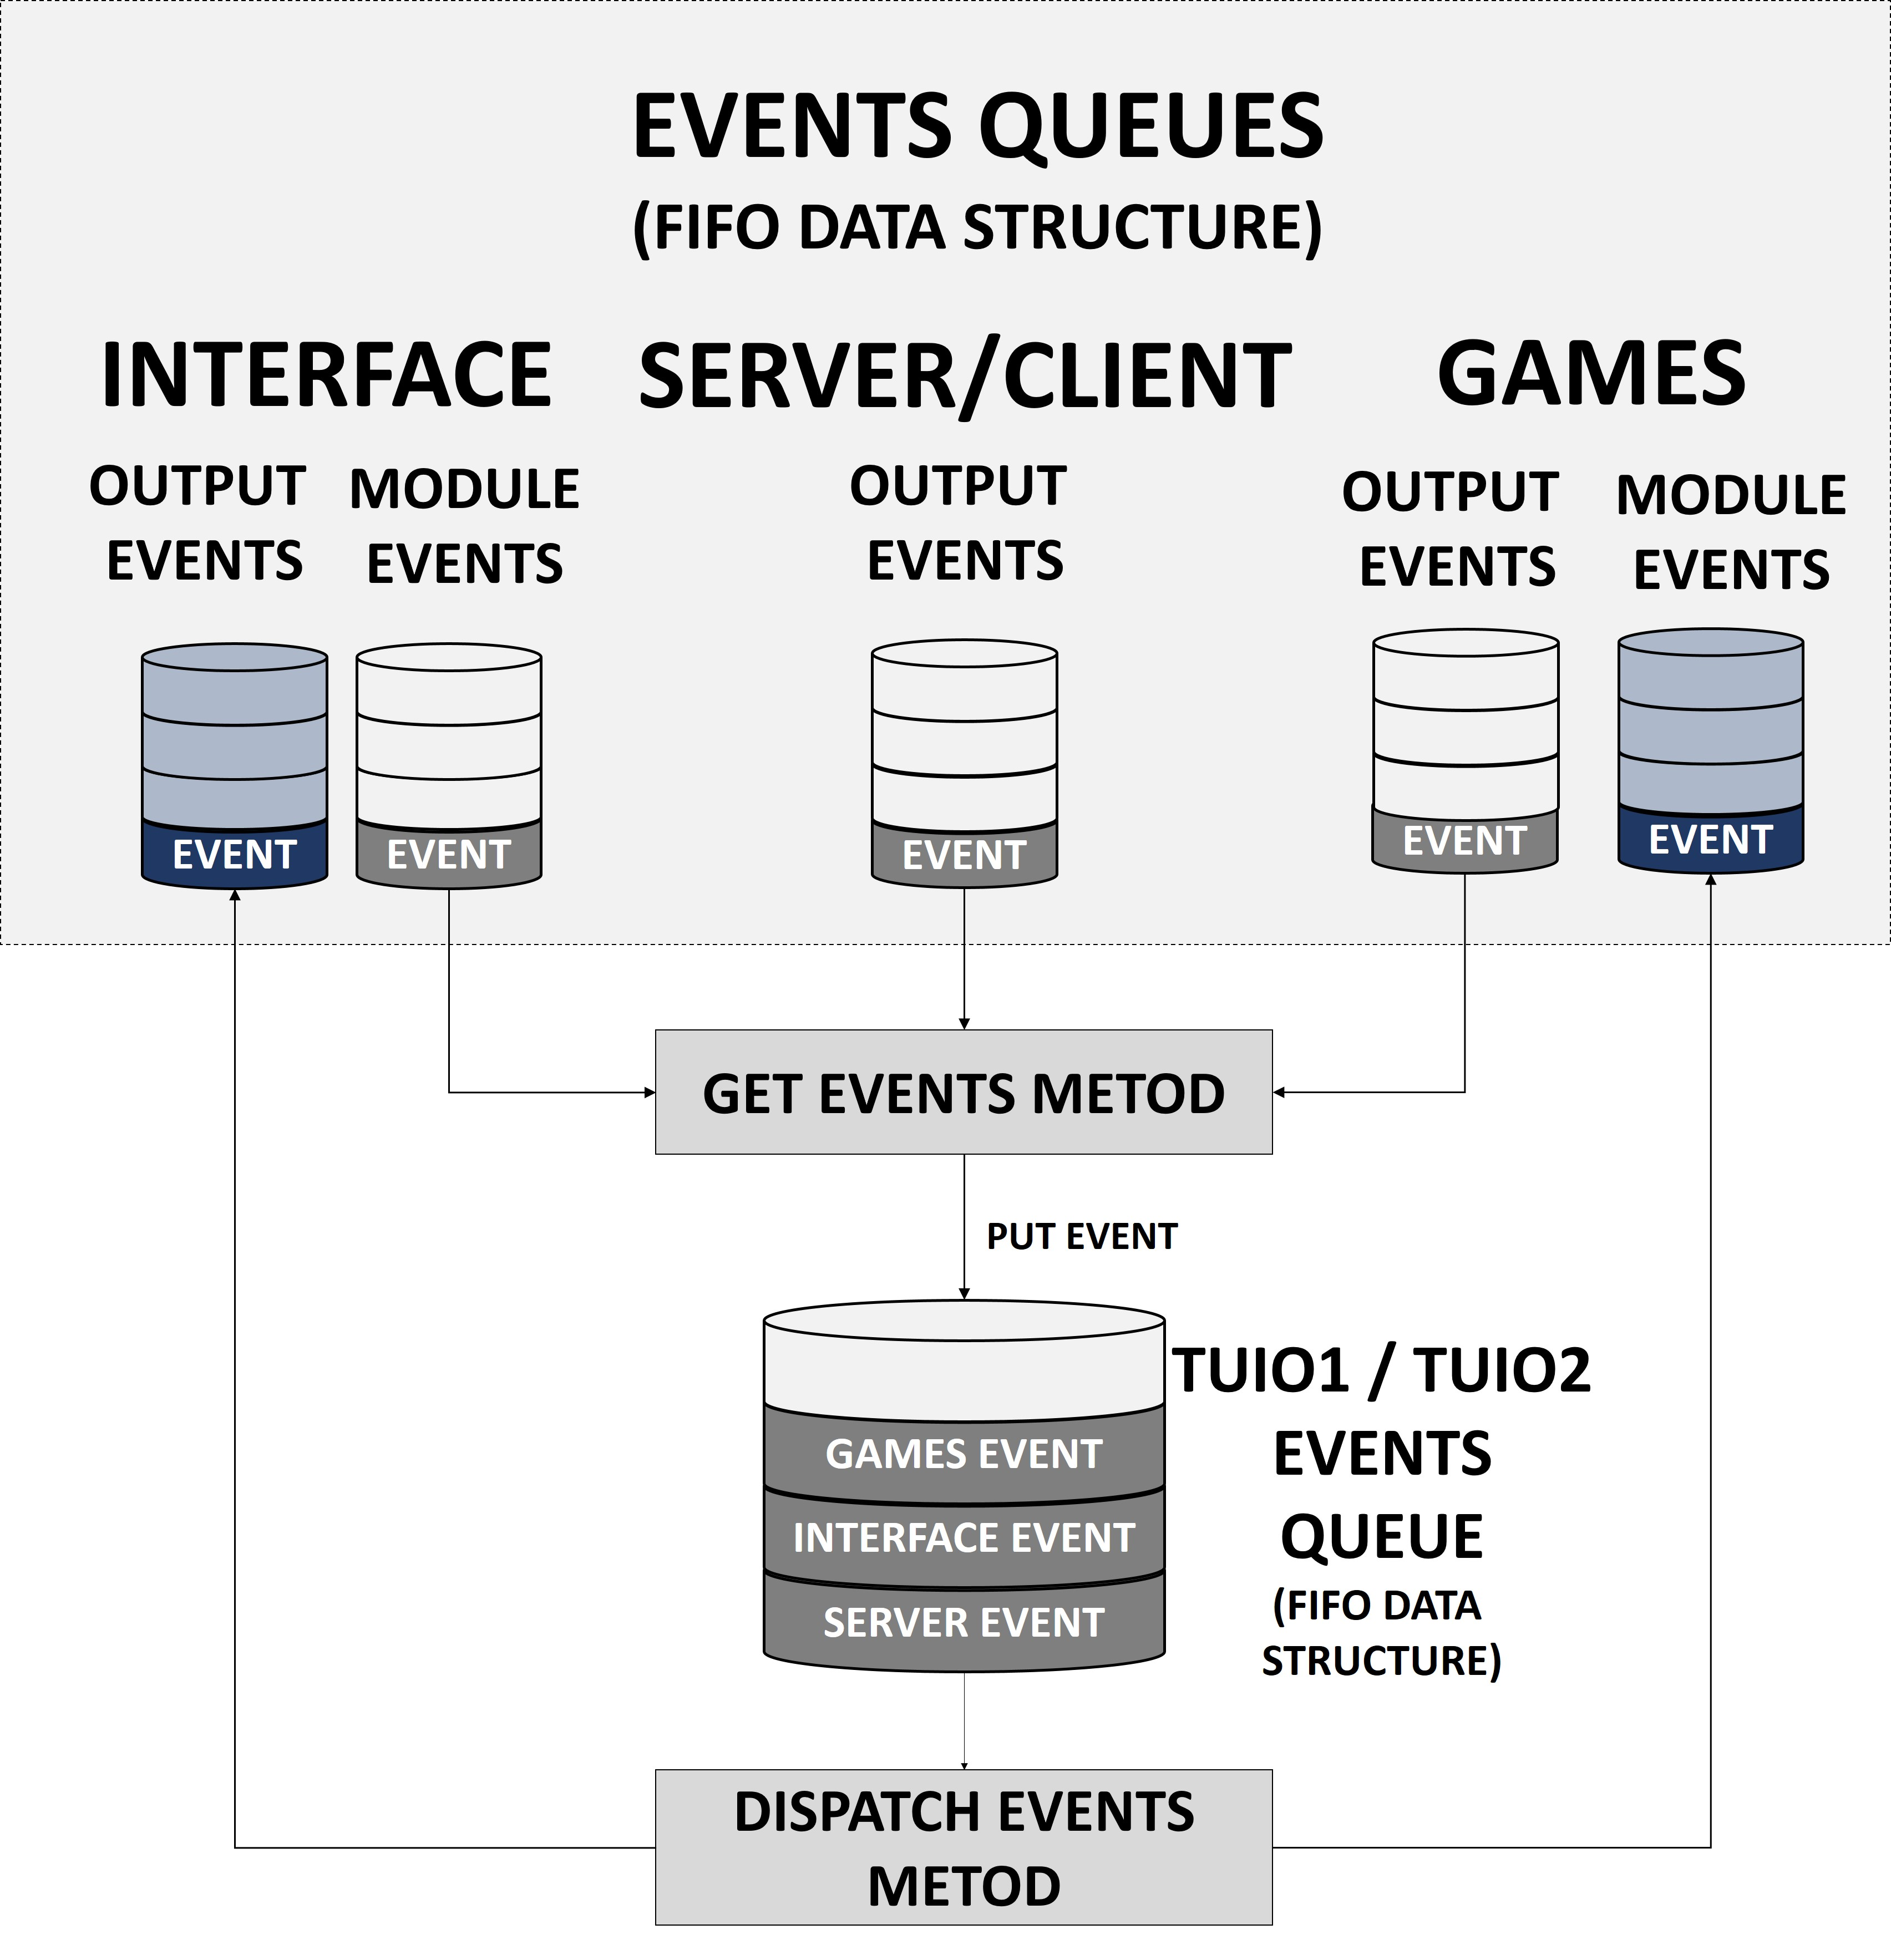
\includegraphics[width=0.9\textwidth]{events_queue.jpg}
\caption{Manejo de eventos en \emph{TUIO1/TUIO2}.}
\label{fig:eventosqueue}
\end{center}
\end{figure}


\subsection{Máquina de estados finitos dispositivo \emph{TUIO1/TUIO2}.}

\subsubsection{IDLE:} Estado inicial del dispositivo \emph{TUIO1/TUIO2}. La máquina permanece en este estado hasta recibir confirmación de comunicación con el dispositivo \emph{TUIO2/TUIO1}.
\subsubsection{MAIN:} Estado principal de la aplicación una vez establecida la comunicación entre los dispositivos \emph{TUIO1} y \emph{TUIO2}.
\subsubsection{GAME:} El dispositivo comienza a ejecutar el juego, al recibir un evento de comenzar juego, desde servidor o cliente.
\subsubsection{EXIT:} Estado de la máquina por el cual se finaliza toda la aplicación.

En la Figura ~\ref{fig:fsmtuio} se muestra la estructura de la máquina de estados, transiciones y métodos de los dispositivos \emph{TUIO1/TUIO2}.

\begin{figure}[!h]
\begin{center}
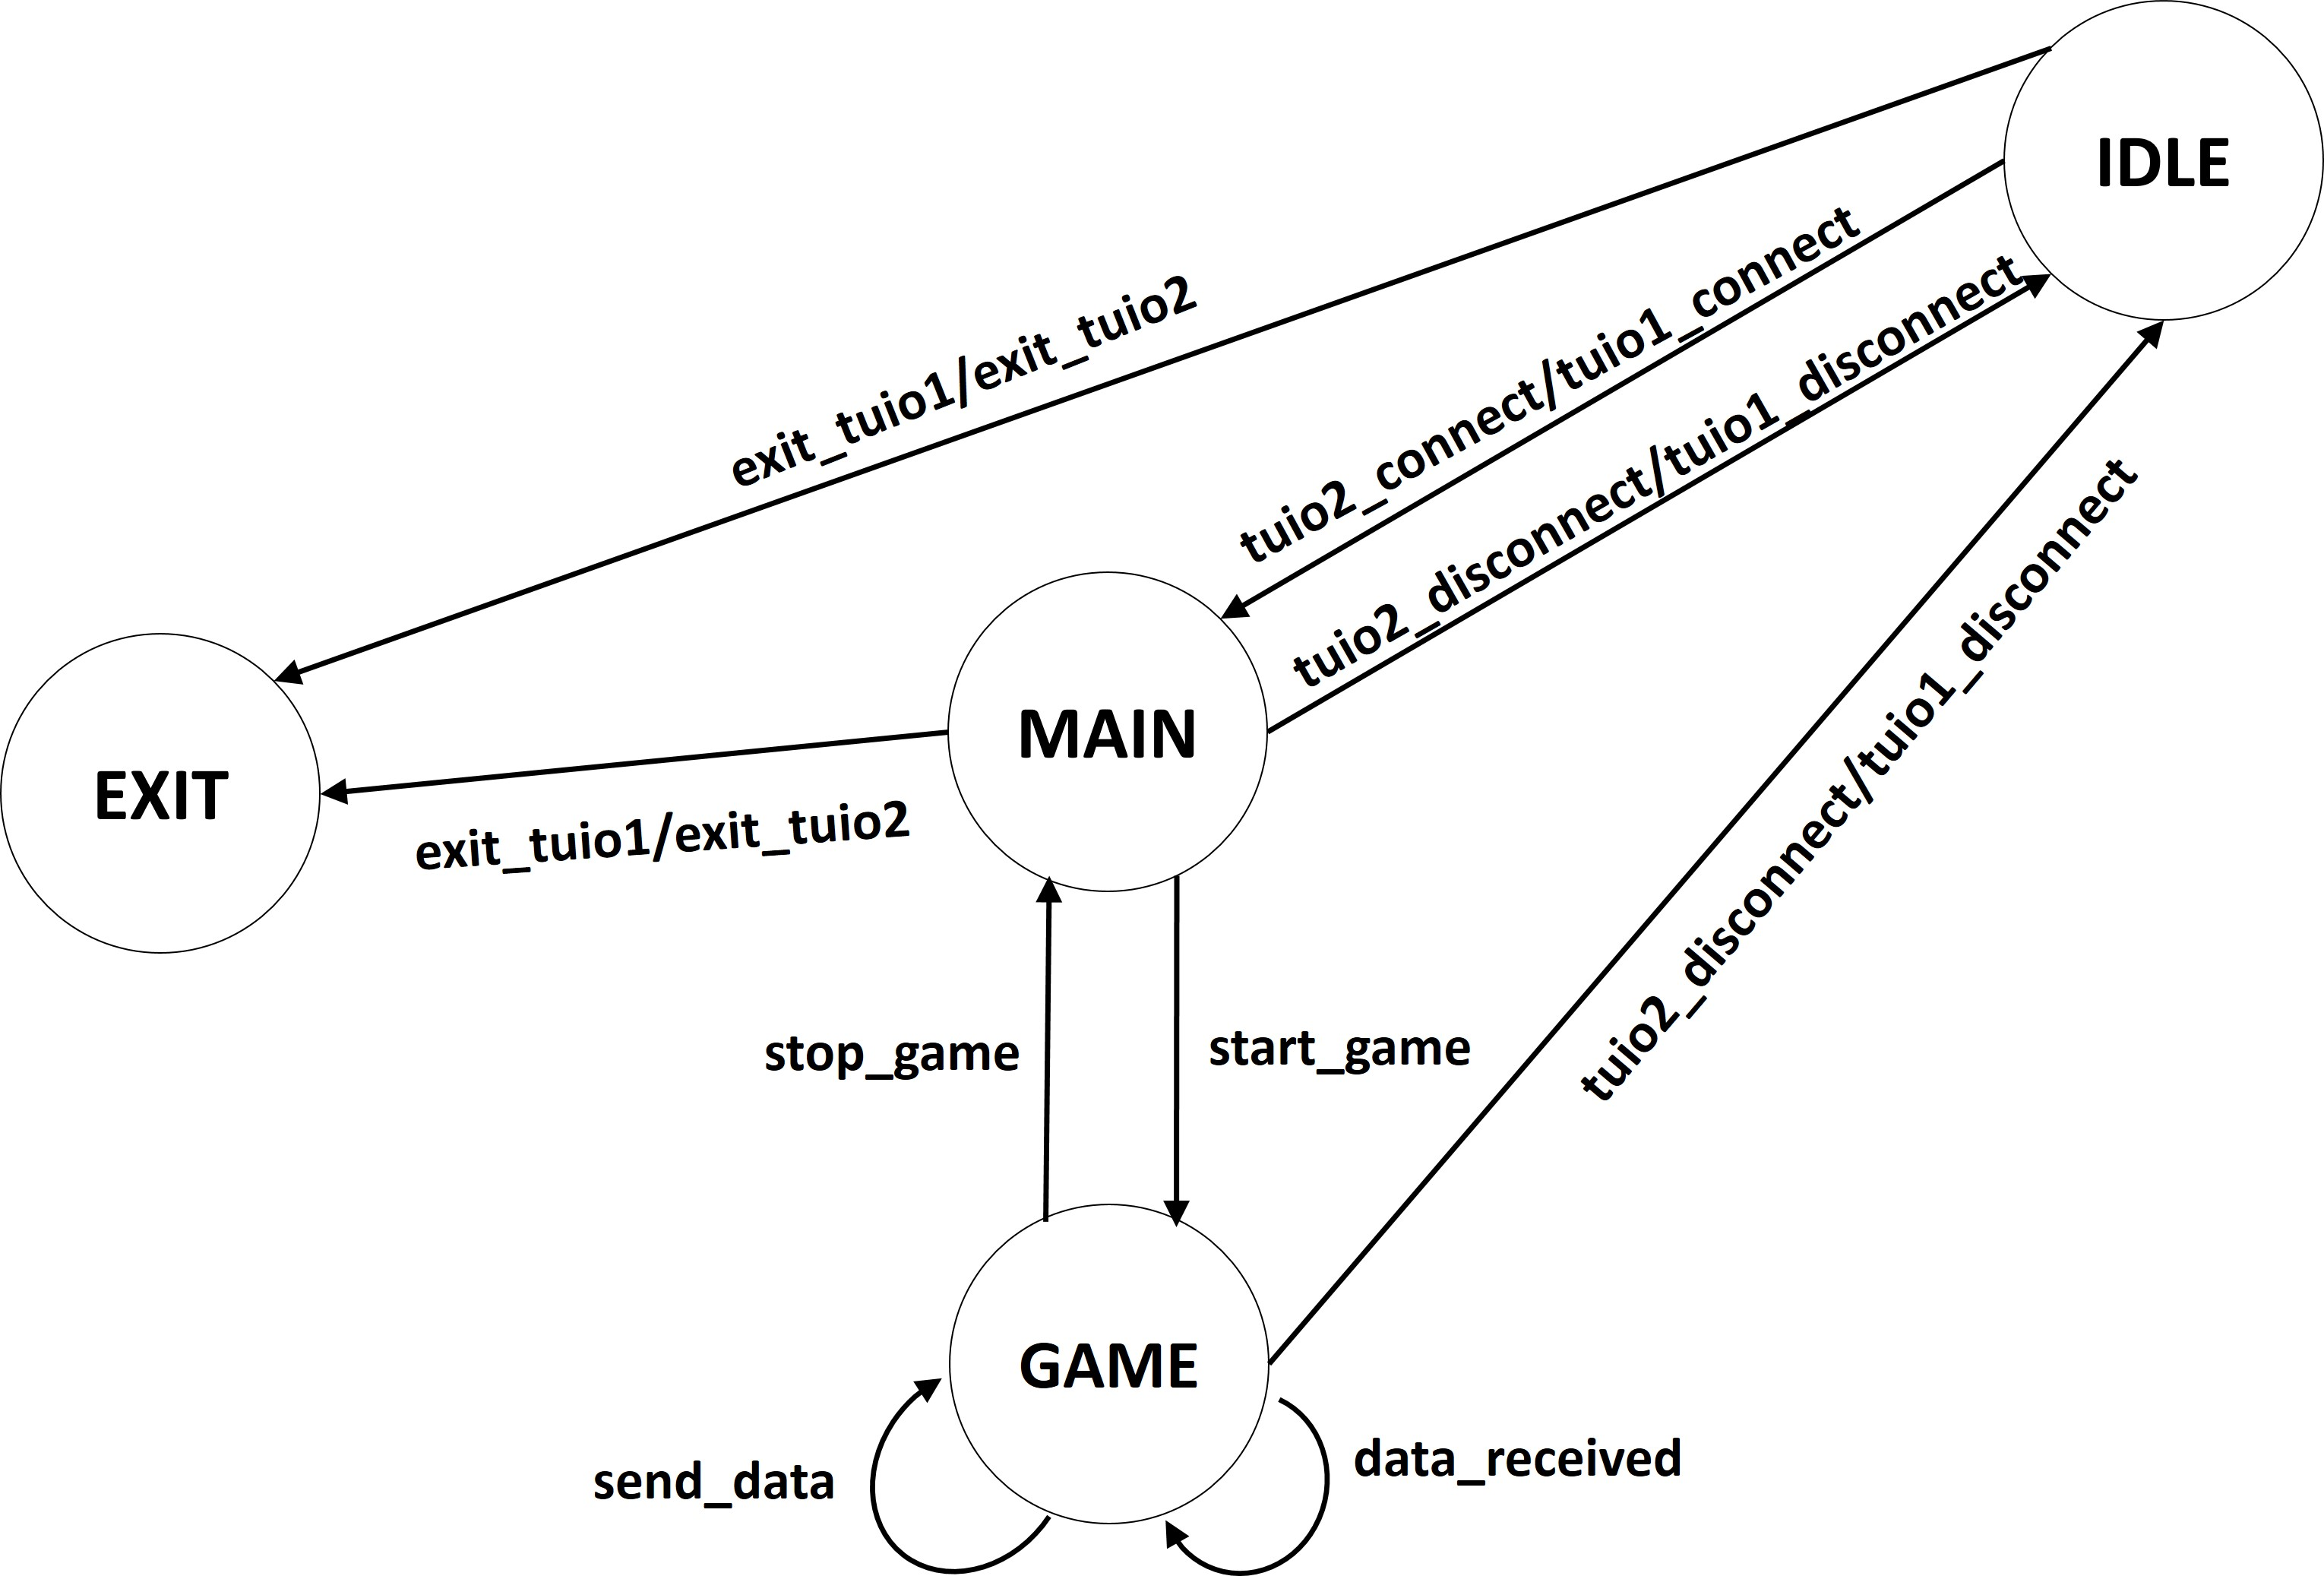
\includegraphics[width=1\textwidth]{fsm_tuio.jpg}
\caption{Estructura máquina de estados finitos \texttt{Tuio1FSM/Tuio2FSM}.}
\label{fig:fsmtuio}
\end{center}
\end{figure}


\subsubsection{Módulos de control \texttt{Tuio1.py/Tuio2.py}}

Estos módulos adquieren y distribuyen los eventos generados en las comunicaciones, interfaz gráfica y juegos, a la parte de la aplicación que corresponda siguiendo la estructura de eventos explicada en el punto anterior.
Los eventos tienen una estructura de \emph{tupla} de tres elementos. Dos de tipo \emph{string}, que indican el tipo de evento y la acción a realizar dentro de la aplicación, y otra \emph{tupla}, de cuatro valores tipo \emph{float}, para los datos obtenidos de los sensores.

\subsubsection{Módulo \texttt{Enum}. Librería estándar de \emph{Python}.}
Método de importación: ~\texttt{from enum import Enum}.

Una enumeración es un conjunto de nombres simbólicos (miembros) vinculados a valores únicos y constantes. Dentro de una enumeración, los miembros se pueden comparar por identidad, y la enumeración misma se puede repetir.

Referencia oficial (24/05/2018):  https://docs.python.org/3/library/enum.html

\subsubsection{Módulo \texttt{Clock}. Librería \emph{Kivy}.}
Método de importación: ~\texttt{from kivy.clock import Clock}

El objeto \texttt{Clock} permite programar una llamada a función una vez o repetidamente, en intervalos especificados. Puede obtener el tiempo transcurrido entre la programación y la llamada de la devolución de llamada mediante el argumento \emph{dt}.

Referencia oficial (24/05/2018):  https://kivy.org/docs/api-kivy.clock.html

\subsubsection{Módulo \texttt{Queue}. Paquete \texttt{multiprocessing} de la librería estándar de \emph{Python}.}
Método de importación: ~\texttt{from multiprocessing import Queue}

Módulo implementado en la programación con hilos, cuando la información debe intercambiarse de forma segura entre múltiples hilos. La clase \texttt{Queue} en este módulo, implementa todas las semánticas de bloqueo requeridas. Las primeras tareas agregadas son las primeras recuperadas (datos \emph{FIFO}).
 
Referencia oficial (24/05/2018): https://docs.python.org/2/library/queue.html

\subsubsection{Módulo \texttt{Thread}. Paquete \texttt{threading} de la librería estándar de \emph{Python}.}
Método de importación: ~\texttt{from threading import Thread}

Este módulo proporciona primitivas de bajo nivel para trabajar con varios subprocesos (también denominados procesos o tareas ligeros ): múltiples hilos de control que comparten su espacio de datos global. Para la sincronización, se proporcionan bloqueos simples (también denominados \emph{mutexes} o \emph{semáforos binarios} ).

Referencia oficial (24/05/2018):  https://docs.python.org/2/library/threading.html

\subsubsection{Módulos propios: \texttt{Server/Client, InterfaceManagement, Games}. Paquete \texttt{lib} de la aplicación.}
Método de importación: \texttt{from lib import Server/Client, InterfaceManagement, Games}

El módulo \texttt{Server/Client} proporciona los métodos para el intercambio de datos entre servidor y cliente.
El módulo \texttt{InterfaceManagement} implementa las funciones y métodos para el manejo de pantallas (\texttt{ScreenManager}) dentro de la aplicación, que ofrece la interfaz gráfica de usuario.
\texttt{Games} está compuesto por las clases y métodos de clase, de juegos básicos de la plataforma, donde serán añadidos los eventos propios para la ejecución de cada uno de ellos.

\subsection{Clases y métodos del módulo \texttt{Tuio1.py/Tuio2.py}.}

\subsubsection{Clase \texttt{Tuio1State()/Tuio2State()}.}
En esta clase son enumerados los distintos estados de la máquina de estados finitos de la aplicación. Hereda del módulo \texttt{Enum}.

\texttt{IDLE = 0  \# Estado inicial de la maquina de estados. Sin comunicaciones.}

\texttt{MAIN = 1  \# Estado principal de la aplicación. Comunicaciones establecidas.}

\texttt{GAME = 2  \# Juego activo.}

\texttt{EXIT = 3  \# Estado final de la aplicación.}

\subsubsection{Métodos de clase \texttt{Tuio1FSM()/Tuio2FSM()}. Transiciones de estado.}

\textbf{Método\texttt{\_\_init\_\_()}}

Establece el estado inicial del objeto al ser instanciado. 

\textbf{Inicialización de los atributos de clase.}

\begin{itemize}
\item \texttt{current}. Atributo que determina el estado de la máquina.
\item \texttt{server/client}. Instancia objeto \texttt{Server/Client}, para las comunicaciones con el cliente/servidor.
\item \texttt{interface}. Instancia objeto \texttt{InterfaceManagement}, que controla los eventos gráficos de la aplicación.
\item \texttt{games}. Instancia al objeto \texttt{Games} para los eventos gráficos, y ejecuta los métodos de los juegos de la aplicación.
\item \texttt{events}. Cola de eventos de la clase \texttt{Tuio1FSM/Tuio2FSM}, donde son añadidos los diferentes eventos de los módulos \texttt{Server/Client, InterfaceManagement} y \texttt{Games}.
\item Llamada al método \texttt{init\_plataform()}, que inicializa las comunicaciones e interfaz gráfica de la plataforma. 
\item Llamada al método \texttt{thread\_get\_event()}, para iniciar el hilo de manejo de eventos.
\end{itemize}

\textbf{Método \texttt{start\_thread\_get\_event()}}.

Llamada al método \texttt{Thread}. Inicia el hilo que contiene el método de reloj cíclico, que obtiene los eventos de los diferentes módulos que componen la aplicación.

\textbf{Método \texttt{thread\_get\_event()}}.

Este método implementa la función reloj (\texttt{clock}), que ejecuta de forma cíclica, el método \texttt{get\_event()}, el cual obtiene los eventos de la aplicación.

\textbf{Método \texttt{get\_event()}}.

Estructura de control que obtiene los eventos de los módulos servidor/cliente, interfaz y juegos.
Estos eventos son añadidos a la cola \texttt{events} del propio módulo, para ser gestionados por el método \texttt{dispatch\_event()}.

\textbf{Método \texttt{dispatch\_event()}}.

Argumento de entrada: \texttt{event}.

Estructura de control para distribuir los eventos a los diferentes métodos, según la transición de estado en la máquina.

\textbf{Método \texttt{init\_plataform()}}.

Llamada a los métodos \texttt{thread\_init\_server()/client(), interface.init\_interface()}, que inicializan los objetos servidor e interfaz.

\textbf{Método \texttt{start\_game()}}.

Argumento de entrada: \texttt{game}.

Método que añade a la cola de eventos del objeto \texttt{game}, para iniciar el juego según el argumento de entrada.

\textbf{Método\texttt{stop\_game()}}.

Argumento de entrada: \texttt{game}.

Método que añade a la cola de eventos del objeto \texttt{game}, para detener el juego según el argumento de entrada.

\textbf{Métodos \texttt{exit\_tuio1()/exit\_tuio2()}}.

Transición al estado máquina \texttt{EXIT}.
Finaliza las comunicaciones, interfaz gráfica y juegos.
Llamada a los métodos \texttt{close\_server()/client()} del objeto \texttt{server/client}, y \texttt{Clock.unschedule} para terminar la ejecución cíclica de adquisición de eventos.

\textbf{Métodos \texttt{tuio2\_connect()/tuio1\_connect()}}.

Método que indica que se han establecido las comunicaciones con el cliente/servidor. Ejecuta un cambio de pantalla (screens) en la interfaz gráfica.

Transición del estado \texttt{IDLE} al estado \texttt{MAIN}.

Llamada al método \texttt{main\_state()} del objeto \texttt{interface}.

\textbf{Métodos \texttt{tuio2\_disconnect()/tuio1\_discconnect()}}.

Método para indicar que se han establecido las comunicaciones con el cliente/servidor.

Transición del estado \texttt{IDLE} al estado \texttt{MAIN}.

Llamada al método \texttt{main\_state()} del objeto \texttt{interface}, que ejecuta un cambio de pantalla en la interfaz gráfica.


\subsection{Gestión de eventos. Pruebas de validación.}

Prueba para las comunicaciones y manejo de eventos entre \emph{TUIO1} y \emph{TUIO2}. 

Ejemplo de proceso de manejo de eventos para comenzar un juego, partiendo del estado \textbf{MAIN} en ambas máquinas de estados (ver Figura~\ref{fig:eventosTUIO2} y Figura~\ref{fig:eventosTUIO1}. 
Pasos seguidos :

Desde la interfaz gráfica de \emph{TUIO2}, se presiona el botón de iniciar juego \textbf{PAINT GAME}. Este evento es de carácter interno del propio módulo \texttt{InterfaceMagmanement} que maneja la interfaz.
El evento pasa por el gestor de eventos de la interfaz gráfica, y es incorporado a la cola de eventos externos, para ser tratado desde el gestor de eventos principal \texttt{Tuio1FSM}. 
El gestor de eventos principal obtiene el evento, el cual es añadido a la cola de eventos dedicada a juegos, para comunicar los datos al cliente, donde es gestionado por el gestor de eventos de \emph{TUIO2}.
El cliente recibe el evento, y lo añade a la cola de eventos del cliente. El gestor principal de eventos \texttt{Tuio2FSM}, lo distribuye, añadiendo las ordenes al gestor de eventos de la interfaz gráfica (\texttt{InterfaceManagement}), y al juego correspondiente para que sea iniciado (\texttt{PaintGame}).

\begin{figure}[!h]
\begin{center}
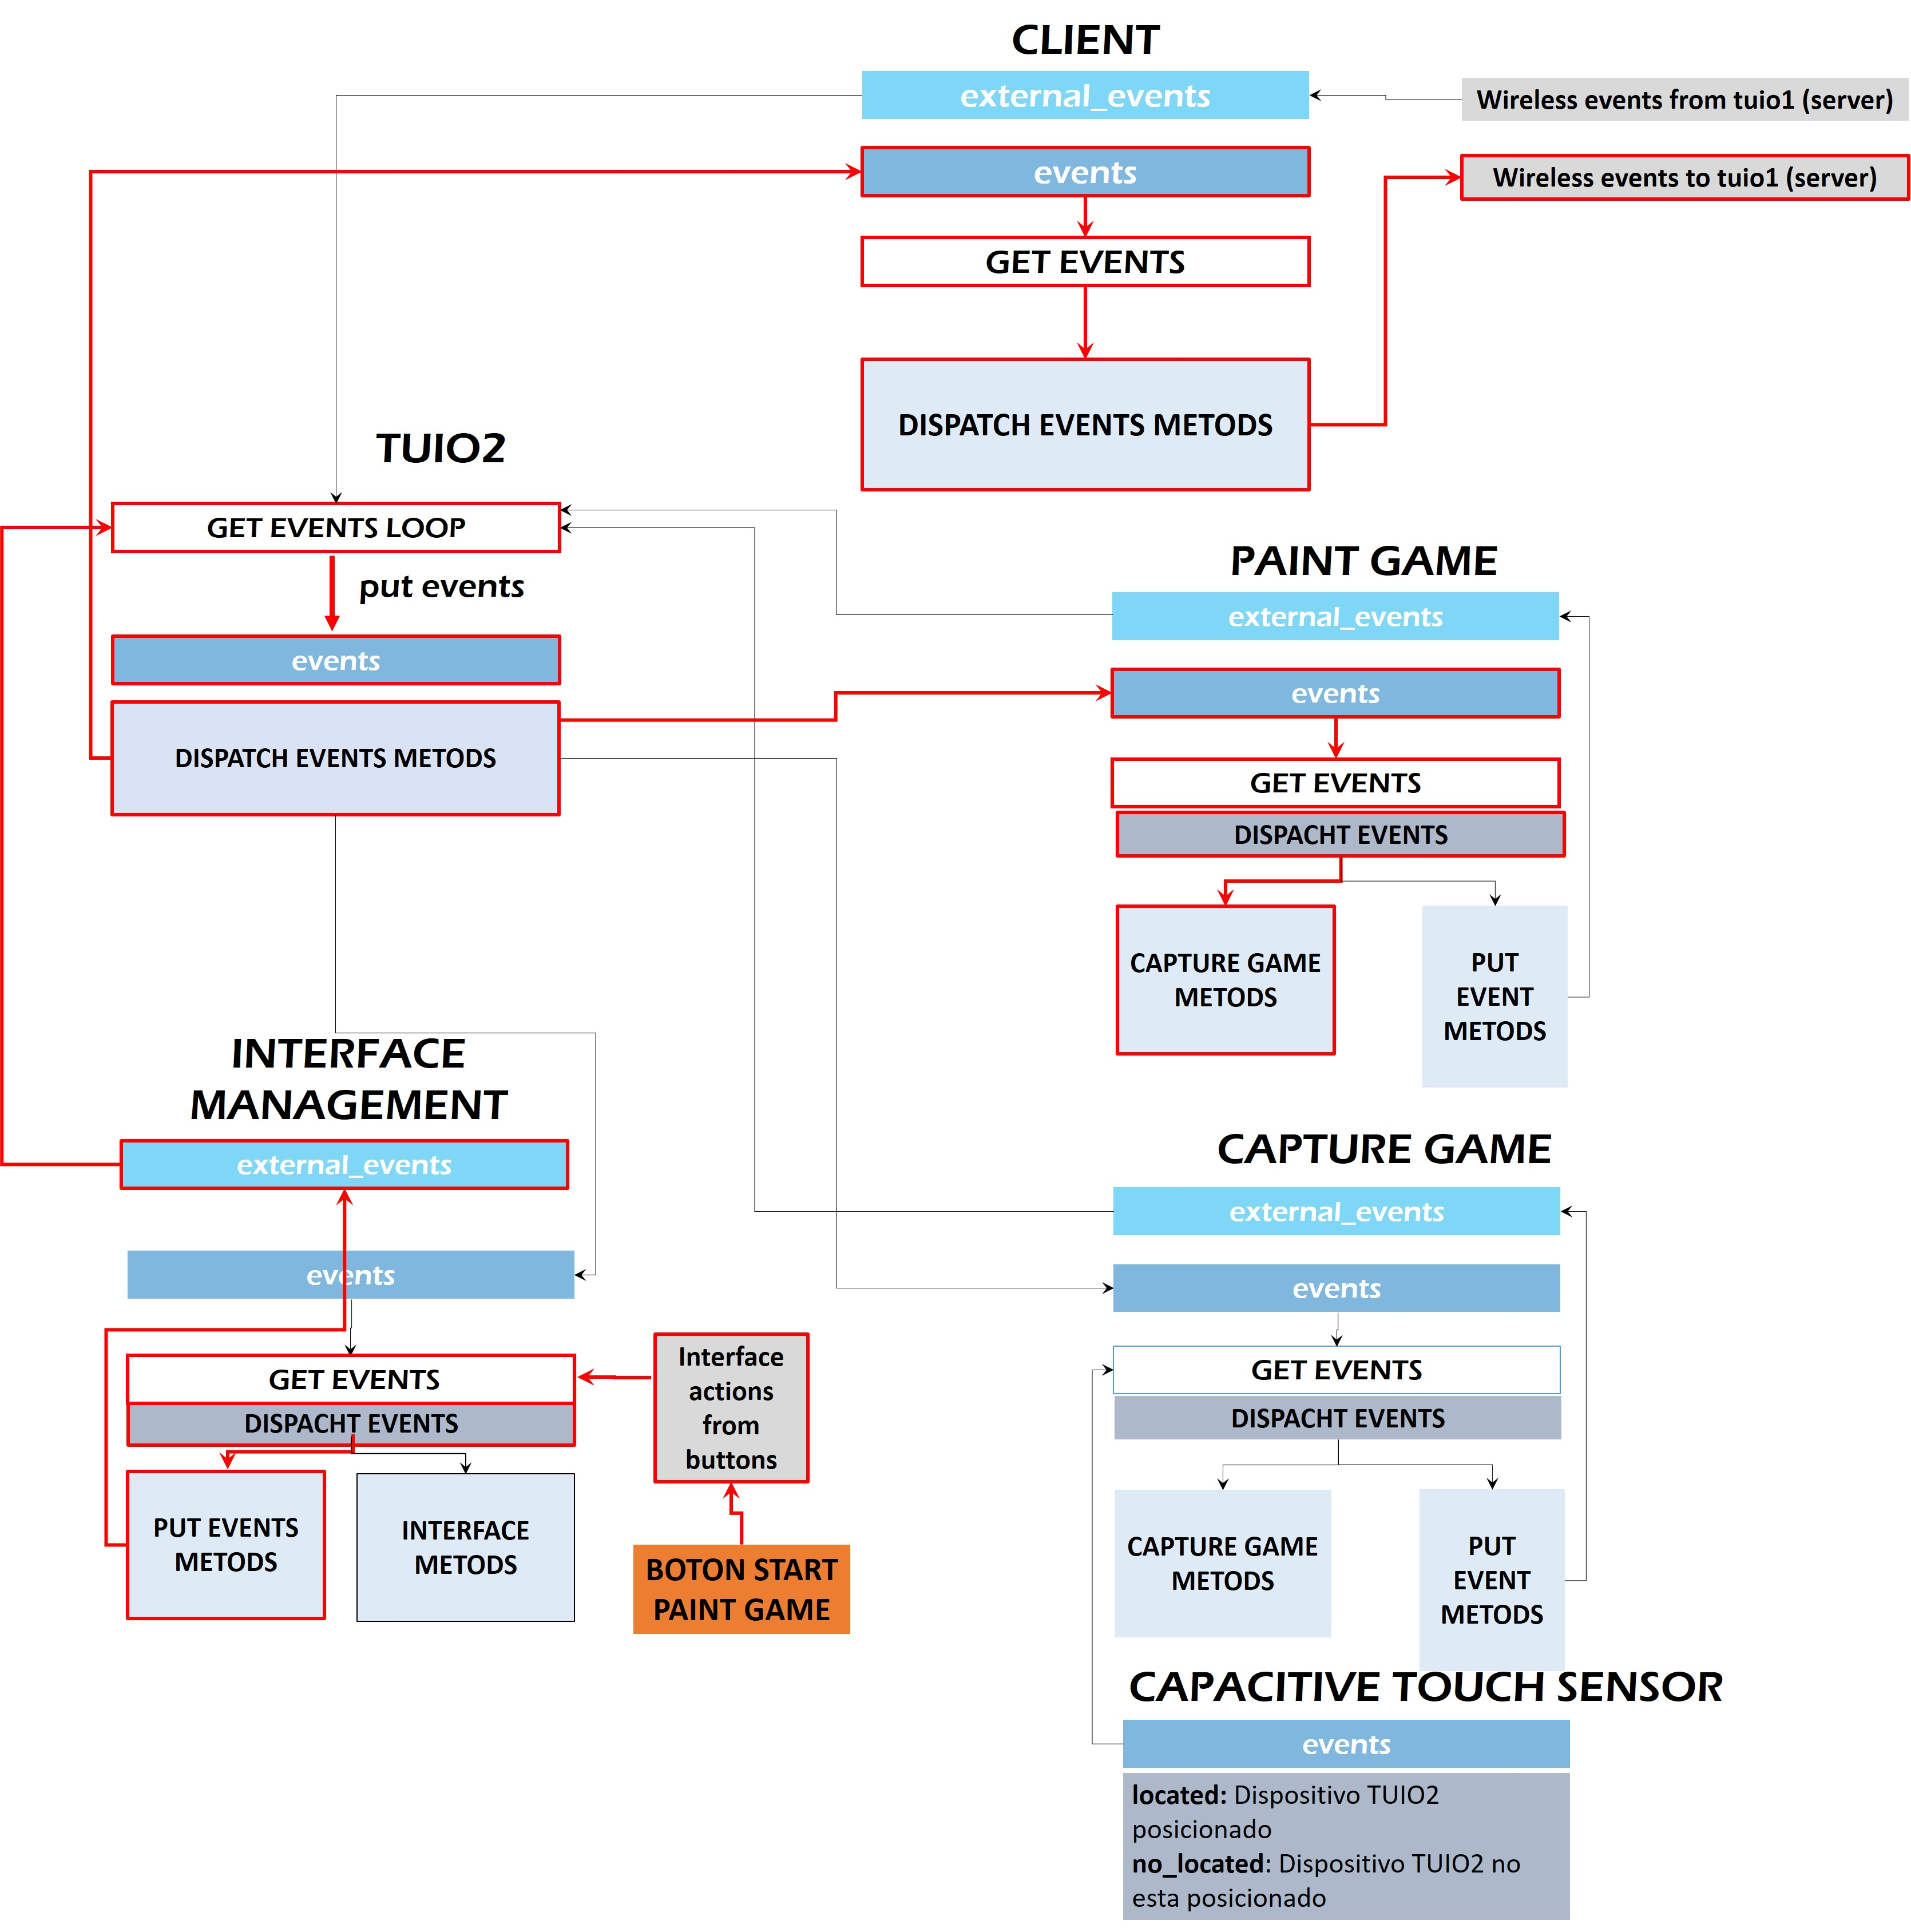
\includegraphics[width=1\textwidth]{events_tuio2.jpg}
\caption{Manejo de eventos en \emph{TUIO2}. Pruebas comenzar juego \textbf{PAINT GAME}.}
\label{fig:eventosTUIO2}
\end{center}
\end{figure}

\begin{figure}[!h]
\begin{center}
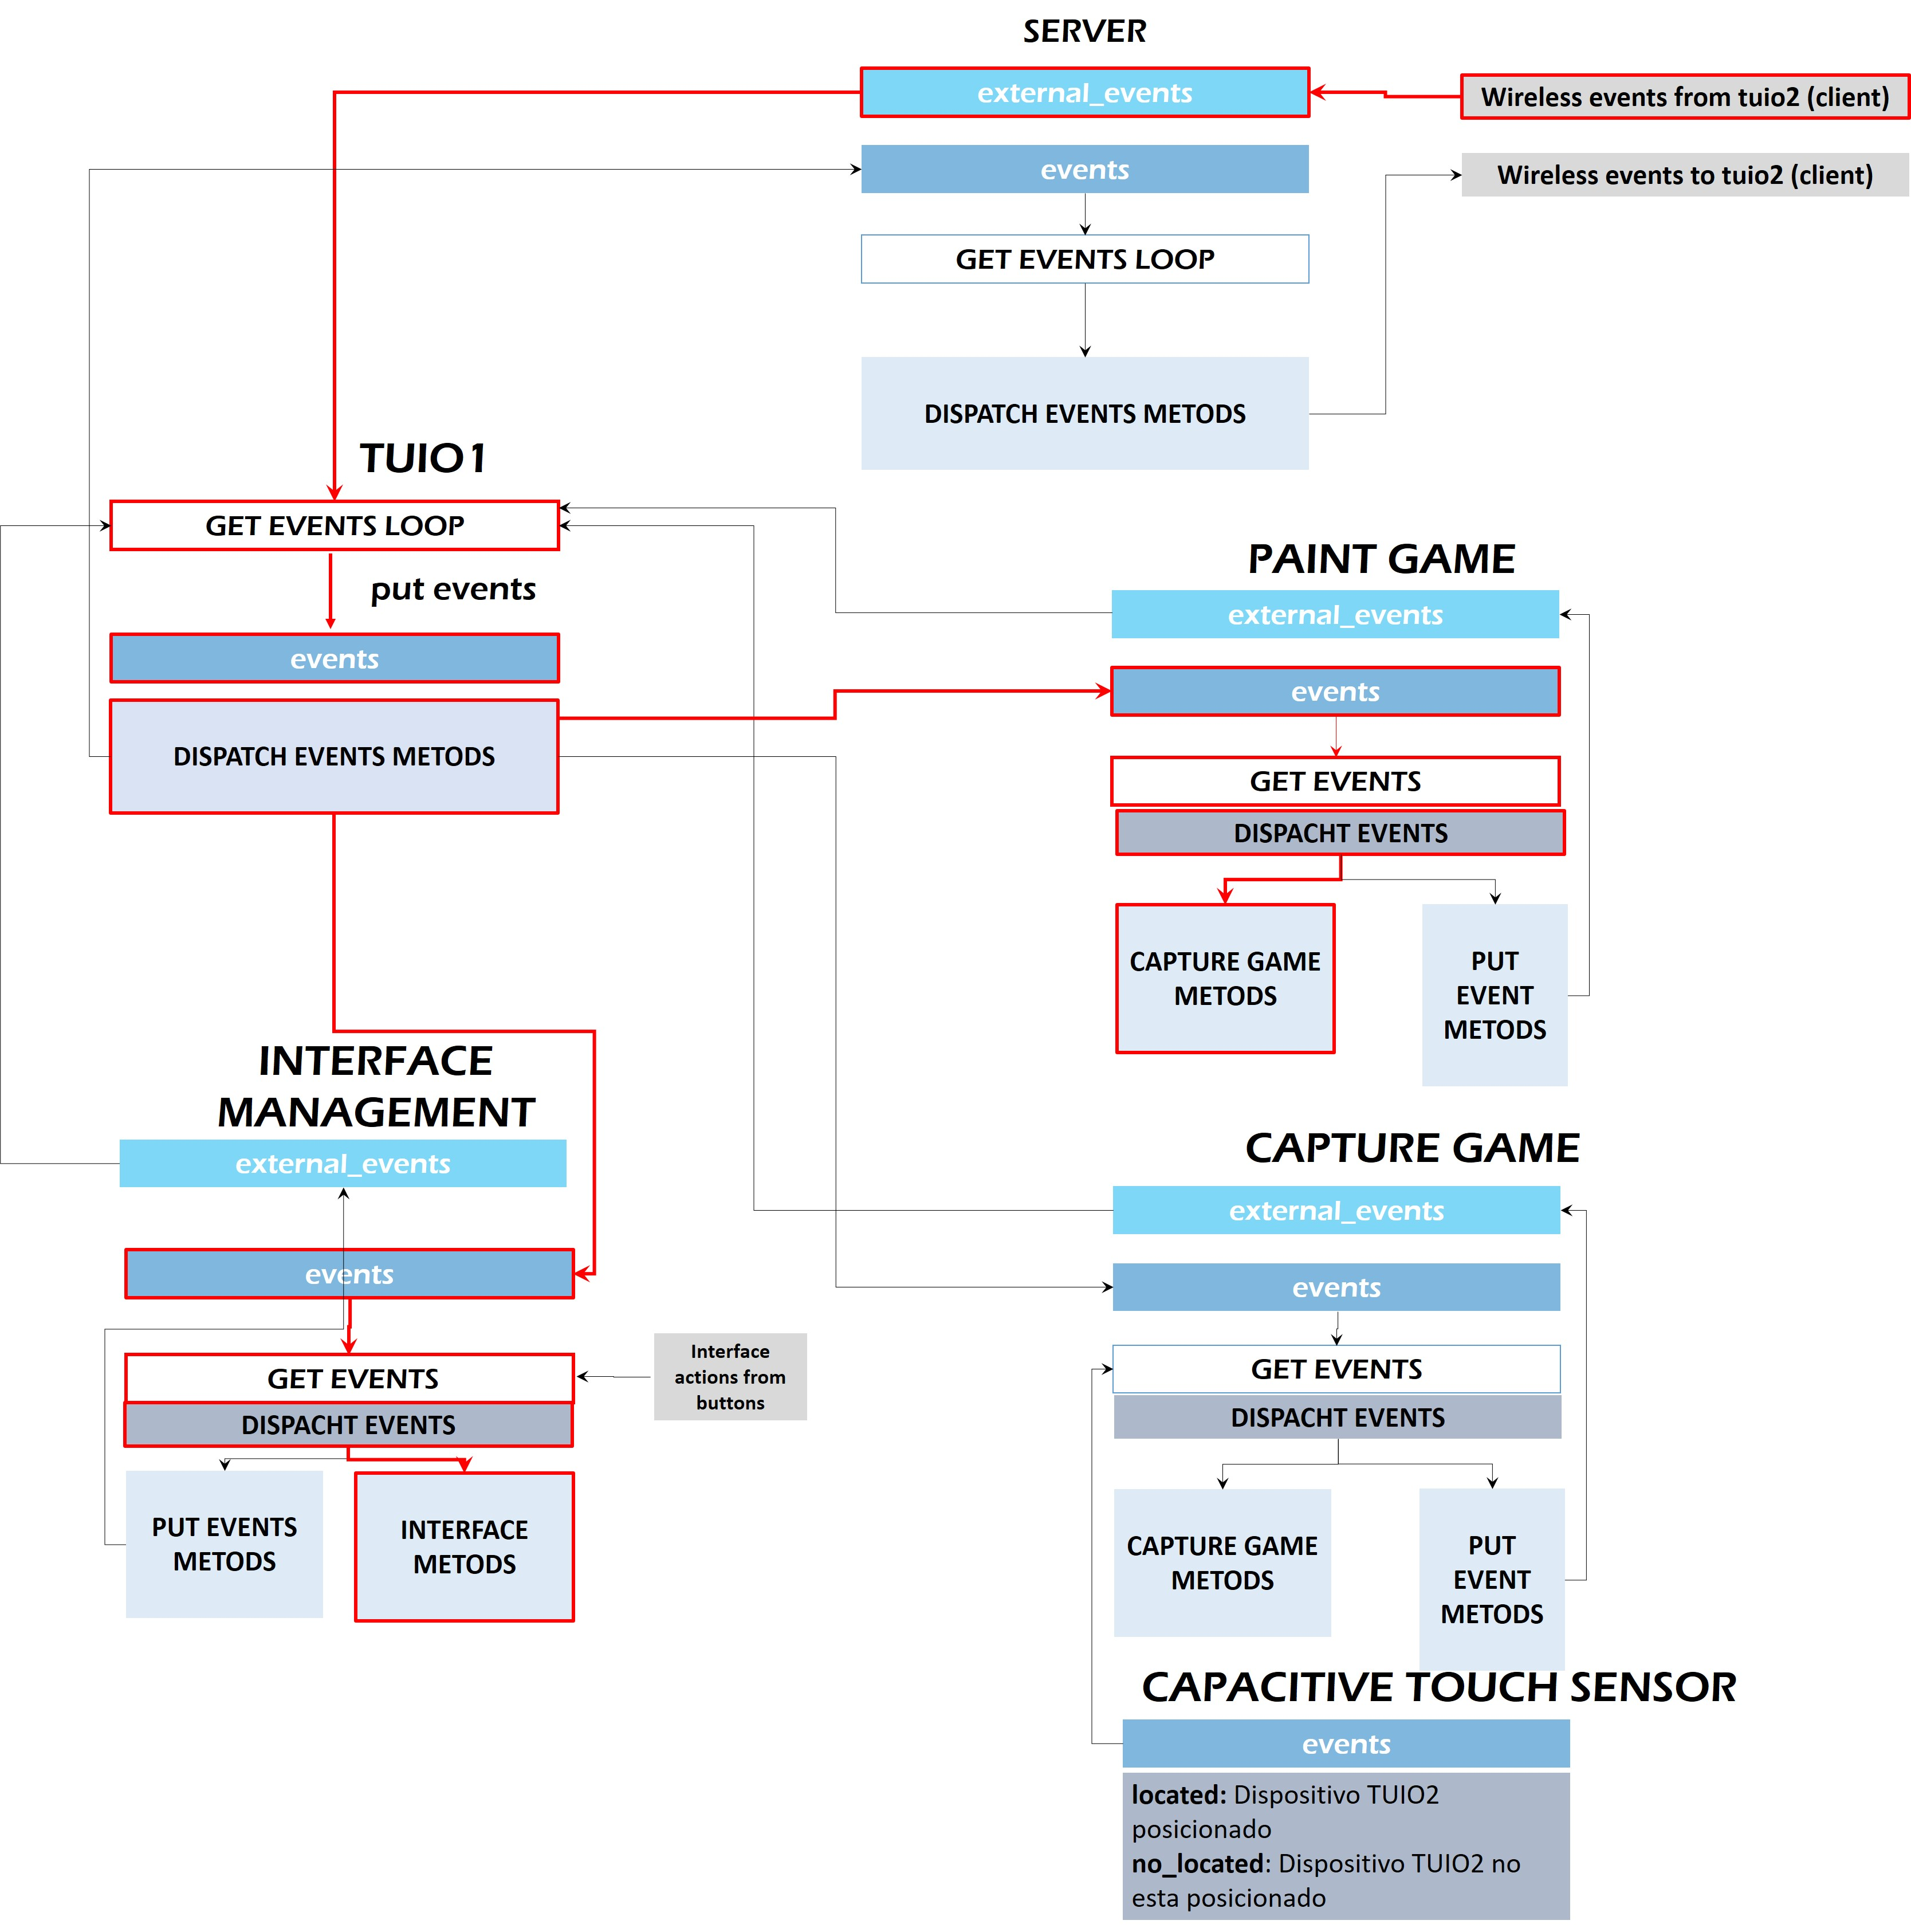
\includegraphics[width=1\textwidth]{events_tuio1.jpg}
\caption{Manejo de eventos en \emph{TUIO1}. Pruebas comenzar juego \textbf{PAINT GAME}.}
\label{fig:eventosTUIO1}
\end{center}
\end{figure}

\subsubsection{Validación del módulo y manejo de eventos \texttt{Tuio1.py} y \texttt{Tuio2.py}.}

La prueba efectuada sobre el manejo de eventos de los módulos principales de la aplicación, han ofrecido resultados correctos en todas las transiciones de estado y ejecución de métodos. Los módulos \texttt{Tuio1FSM} y \texttt{Tuio2FSM} son validados para su utilización dentro de la aplicación. Queda abierta la posibilidad de añadir distintos métodos y transiciones, siempre y cuando no se vea afectada la estructura principal de manejador de eventos.


\section{Comunicaciones Servidor / Cliente.}
\label{sec:comunicaciones}

\subsection{Máquina de estados finitos Servidor / Cliente.}

\textbf{IDLE:} Estado inicial del servidor a la espera de recibir un evento desde la máquina de estados del dispositivo \emph{TUIO1/TUIO2} para iniciar el servidor/cliente.
\textbf{Transiciones/Métodos.}
\begin{itemize}
\item \texttt{init\_server/init\_client:} transición al estado \textbf{LISTEN}. La ejecución de esta transición sucede cuando la máquina de estados del servidor/cliente recibe el evento \texttt{init\_server/init\_client} dentro de la máquina de estados \texttt{ServerFSM/ClientFSM}.

\item \texttt{close\_server/close\_client:} transición al estado \textbf{EXIT} al recibir el evento \texttt{close\_server/close\_client} desde la máquina de estados \texttt{Tuio1FSM/Tuio2FSM}, para cerrar el servidor/cliente.
\item \texttt{create\_server/create\_client}. Entrada desde la máquina de estados \texttt{Tuio1FSM/Tuio2FSM}, al iniciar el dispositivo.
\item \texttt{reconnect}(perdida de conexión). Entrada de evento de reconexión al interrumpirse la conexión con el cliente/servidor.
\item \texttt{reconnect}(tiempo de espera). Agotado tiempo de espera para conectar con \emph{TUIO2/TUIO1}.
\end{itemize}

\textbf{LISTEN:} El servidor/cliente queda a la espera de conectar con (\emph{TUIO2/TUIO1}). En el caso de no conectar con el cliente/servidor (en un tiempo definido de 10 segundos), es ejecutada la transición \texttt{reconnect}. 
Al conectar con \emph{TUIO2/TUIO1} (cliente/servidor), \emph{ServerFSM/ClientFSM} ejecuta la transición \texttt{wait\_data} hasta el estado \textbf{CONNECT}, a la espera de recibir datos desde \emph{TUIO2/TUIO1}.

\textbf{Transiciones/Métodos.}
\begin{itemize}
\item \texttt{reconnect}: la máquina vuelve al estado \textbf{IDLE}, al agotarse el tiempo de espera para conectar con el cliente/servidor. Se crea el evento \emph{init\_client}, para volver a iniciar el servidor/cliente.
\item \texttt{close\_server/close\_client}: transición al estado \textbf{EXIT} al recibir el evento \texttt{close\_server/close\_client} desde la máquina de estados \texttt{Tuio1FSM/Tuio2FSM}, para cerrar las comunicaciones.
\item \texttt{init\_server/init\_client}: el servidor/cliente queda a la espera de conectar con \emph{TUIO2/TUIO1}.
\end{itemize}

\textbf{CONNECT:} Existe comunicación entre los dispositivos \emph{TUIO1} y \emph{TUIO2}. 
Dispone de dos entradas y una transición posible: recibir datos, enviar datos, o volver a iniciar el servidor si la conexión ha sido interrumpida respectivamente.

\textbf{Transiciones/Métodos.}
\begin{itemize}
\item \texttt{reconnect}: la máquina vuelve al estado \textbf{IDLE}, al interrumpirse la comunicación con el cliente/servidor. Se crea el evento \emph{init\_server/init\_client}, para volver a iniciar el servidor/cliente.
\item \texttt{close\_server/close\_client:} transición al estado \textbf{EXIT} al recibir el evento \texttt{close\_server/close\_client} desde la máquina de estados \texttt{Tuio1FSM/Tuio2FSM}, para cerrar las comunicaciones.
\item \texttt{receive\_data}: es ejecutada si se reciben datos desde \emph{TUIO2/TUIO1}. Los datos son añadidos a la cola de eventos de salida, la cual es manejada por \emph{Tuio1FSM/Tuio1FSM} (por medio de \texttt{data\_received}). Se mantiene en el estado \textbf{CONNECT}, a la espera de recibir mas datos desde \emph{TUIO2/TUIO1}.
\item \texttt{send\_data}: método para enviar datos al cliente/servidor.
\end{itemize}
\textbf{EXIT}: Estado de la máquina por el cual se finaliza el servidor/cliente.

\textbf{Transiciones/Métodos.}

\texttt{close\_server/close\_client}: evento de entrada para finalizar las comunicaciones.


La Figura ~\ref{fig:fsmcoms} muestra la estructura de la máquina de estados del servidor/cliente de \emph{TUIO1/TUIO2}.

\begin{figure}[!h]
\begin{center}
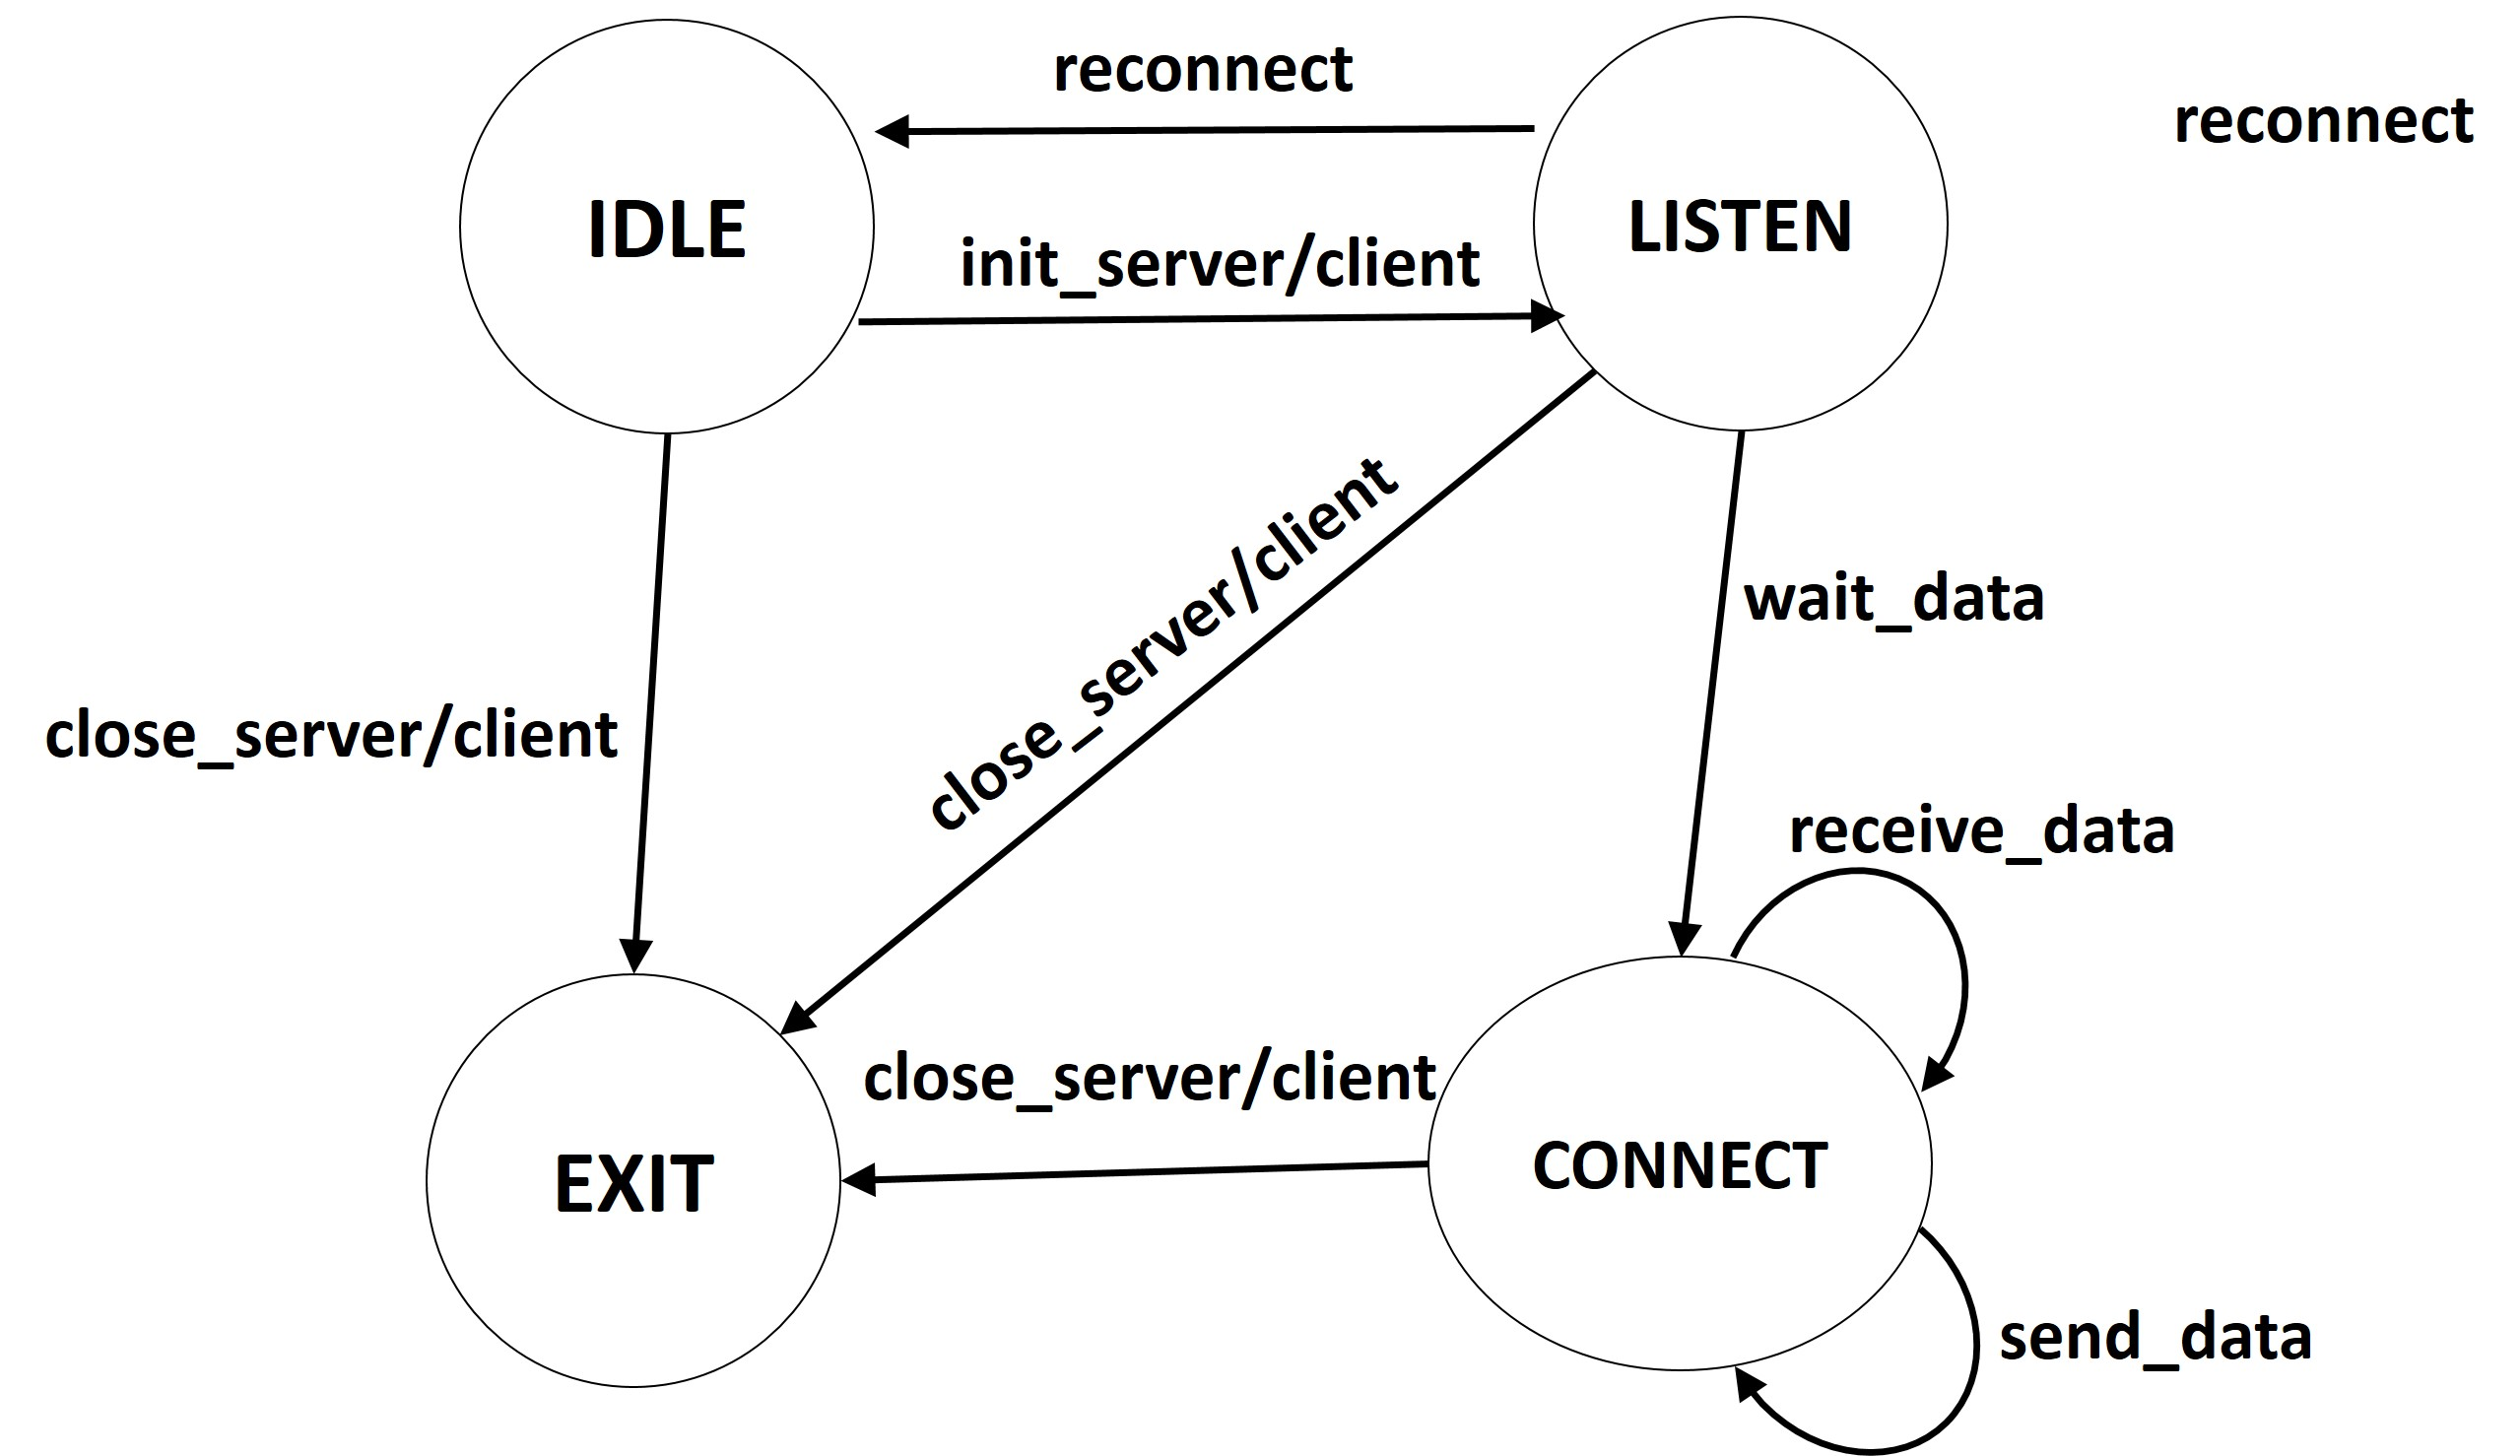
\includegraphics[width=1\textwidth]{fsm_coms.jpg}
\caption{Estructura máquina de estados finitos del servidor/cliente.}
\label{fig:fsmcoms}
\end{center}
\end{figure}

\subsection{Gestión de eventos Servidor/Cliente.}
Los eventos de entrada desde servidor/cliente son añadidos a la cola \texttt{output\_events}, donde son adquiridos por el gestor de eventos de \texttt{Tuio1FSM/Tuio2FSM}, con el método \texttt{send\_event(event)}, donde \texttt{event} es el evento a enviar.
Tanto el servidor como el cliente no disponen de eventos de salida. Para enviar eventos desde un dispositivo a otro, se utilizan los métodos \texttt{server.output\_event.get()/server.output\_event.get()} de clase de \texttt{ServerFSM/ClientFSM}. En la Figura ~\ref{fig:events_serverclient}, se muestra de forma gráfica, la gestión de eventos.
\begin{figure}[!h]
\begin{center}
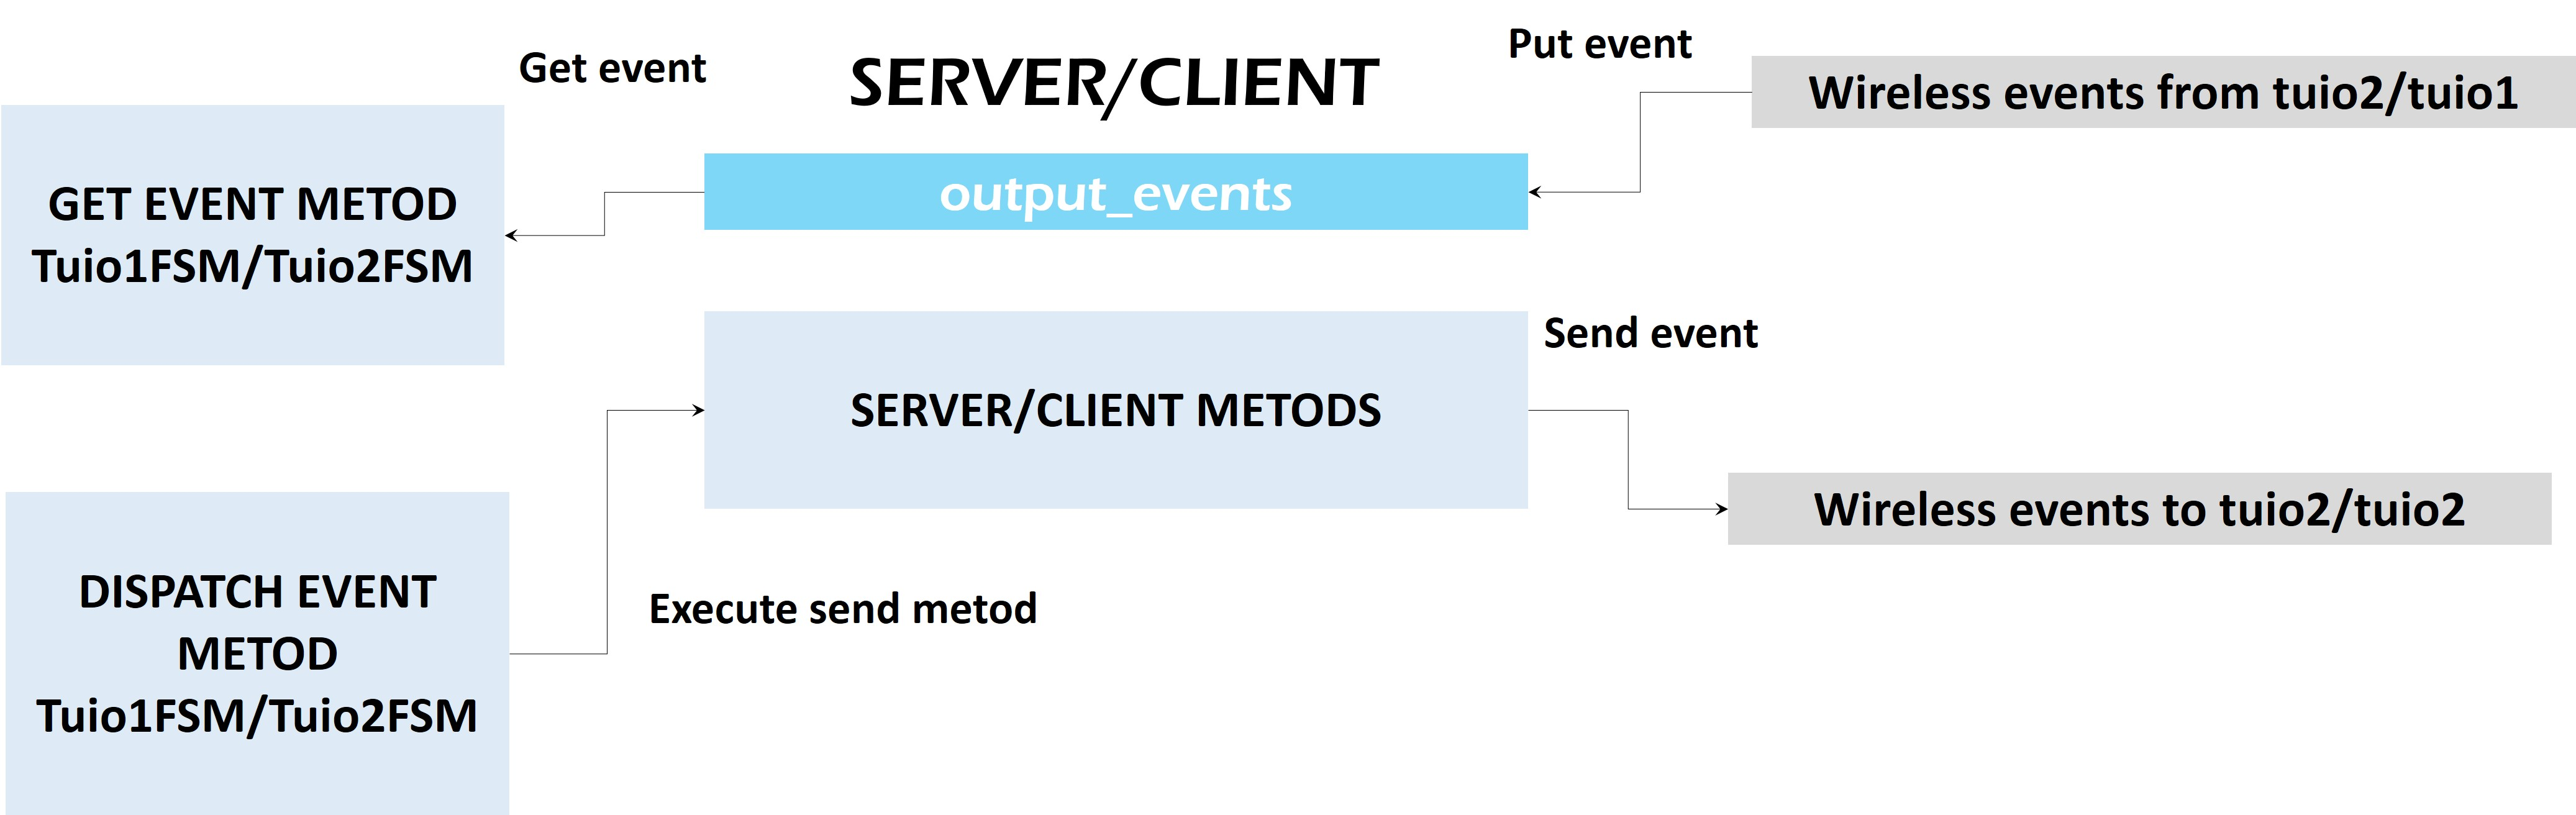
\includegraphics[width=1\textwidth]{events_serverclient.jpg}
\caption{Estructura manejo de eventos Servidor/Cliente.}
\label{fig:events_serverclient}
\end{center}
\end{figure}


\subsection{Pruebas de validación en las comunicaciones cliente-servidor.}

El programa de pruebas consiste en realizar él envió/recepción de datos entre los dispositivos, donde se realizan secuencias básicas en las comunicaciones.
La secuencia del programa de pruebas en las comunicaciones cliente servidor, es la siguiente:

El servidor se inicia en el \emph{puerto 8888} y queda a la espera de la conexión del cliente. Se imprime por pantalla lado servidor: «Esperando cliente». 

Una vez el cliente establece la comunicación con el servidor, se imprime por pantalla en lado servidor: «Cliente conectado». De igual manera, en el lado cliente, se imprime por pantalla: «Conectado a servidor».

Se crea un evento para indicar a ambos dispositivos que se inicie el juego (estado \textbf{GAME}). Se imprime por pantalla el mensaje: «Juego iniciado»

Cuando ambos dispositivos están en el estado \textbf{GAME}, el servidor envía una petición de datos de la unidad de medición inercial \emph{MPU-9255}.

Este evento es gestionado en el programa principal \texttt{tuio2}, que devuelve la petición solicitada del servidor. Se imprime por pantalla: «Datos enviados al servidor.». Son mostrados los datos recibidos en el servidor una vez manejado el evento de entrada: «Datos recibidos del cliente: » 

Es finalizada la conexión y la aplicación de ambos dispositivos, mostrando respectivamente: «Aplicación finalizada»

La Figura ~\ref{fig:fsmexample} muestra de manera gráfica, la secuencia básica expuesta para las pruebas de las comunicaciones.

\begin{figure}[!h]
\begin{center}
\includegraphics[width=1\textwidth]{fsm_example1.jpg}
\caption{Estructura de la secuencia de las pruebas cliente-servidor.}
\label{fig:fsmexample}
\end{center}
\end{figure}


\section{Sistema de localización.}
El sistema de localización consiste en obtener las coordenadas de posición y ángulo, del \emph{Widget tangible TUIO2}, al ser posicionado sobre la pantalla táctil capacitiva del dispositivo \emph{TUIO1}. Estos eventos táctiles siguen un patrón determinado, cuya información es procesada para una interacción gráfica y tangible entre dispositivos.
Son dos las interacciones posibles mediante el sistema de localización: incorporar información gráfica de \emph{TUIO2} a \emph{TUIO1}, o \emph{extraer} información desde \emph{TUIO1} a \emph{TUIO2}.

Para generar estos eventos táctiles, el dispositivo \emph{TUIO2} dispone de tres almohadillas conductoras, que al tomar contacto con la pantalla capacitiva, se generan varios eventos táctiles simultáneos.

\subsection{Versión de pruebas 1. Localización de coordenadas con patrón de triángulo rectángulo escaleno.}  

Ejemplo de aplicación del sistema de localización. Antes de posicionar \emph{TUIO2} sobre \emph{TUIO1}, las pantallas de ambos dispositivos muestran imágenes diferentes (ver Figura~\ref{fig:Localizacion1}).
\begin{figure}[!h]
\begin{center}
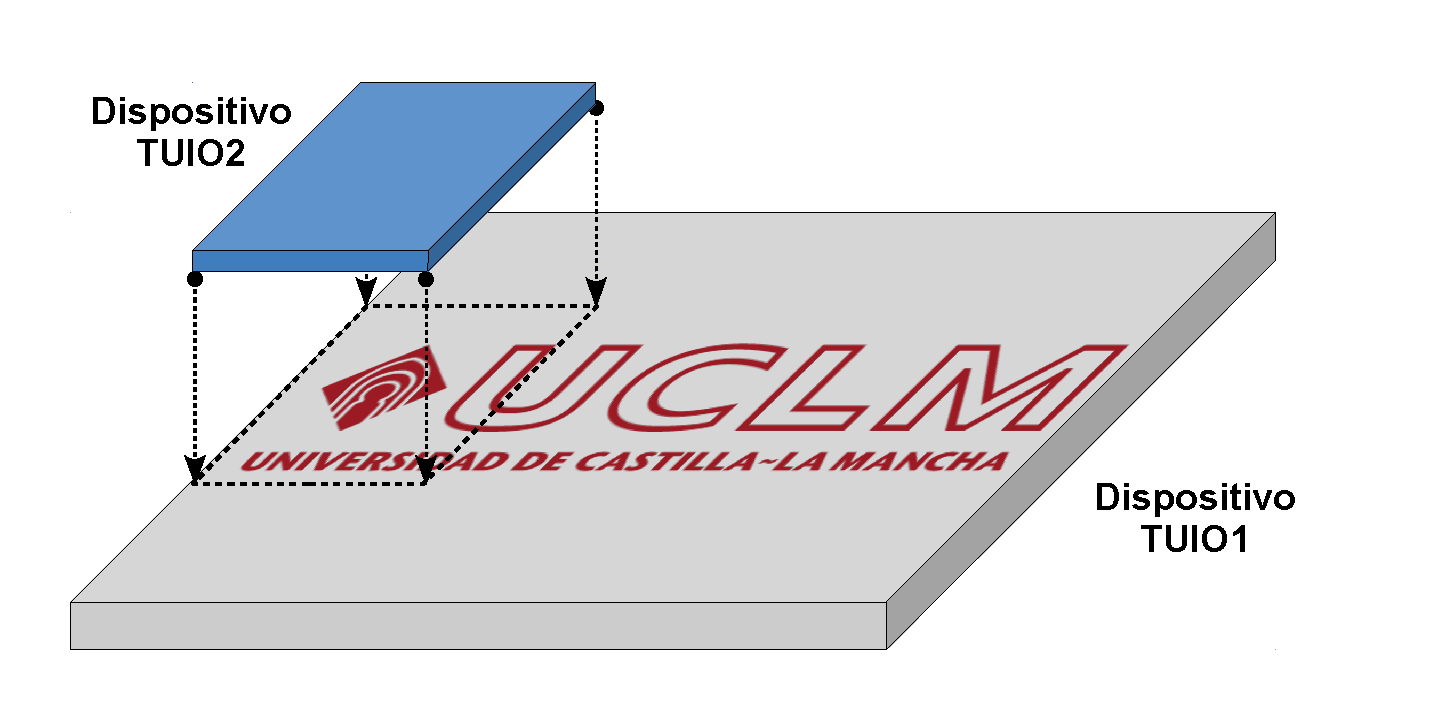
\includegraphics[width=0.7\textwidth]{localizacion1.pdf}
\caption{Versión de pruebas no validas. Posición de los dispositivos antes de la interacción sobre la pantalla capacitiva.}
\label{fig:Localizacion1}
\end{center}
\end{figure}
Al posicionar \emph{TUIO2} sobre la pantalla de \emph{TUIO1}, la pantalla de \emph{TUIO2} muestra la parte de imagen correspondiente que es tapada por el dispositivo. (Figura~\ref{fig:Localizacion2}).
\begin{figure}[!h]
\begin{center}
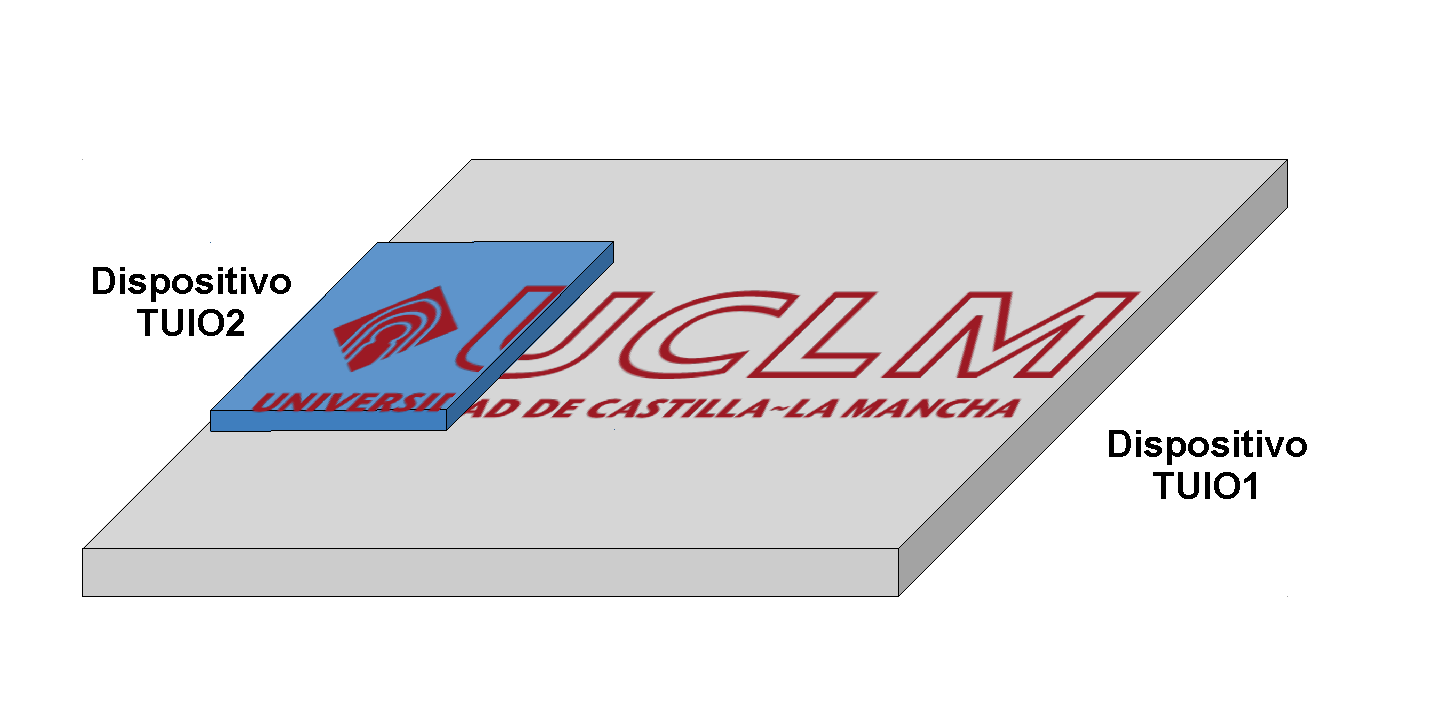
\includegraphics[width=0.7\textwidth]{localizacion2.pdf}
\caption{Versión de prueba no valida. Posición de los dispositivos después de la interacción sobre la pantalla capacitiva.}
\label{fig:Localizacion2}
\end{center}
\end{figure}

El procedimiento para obtener la posición, se consigue con el uso del sensor capacitivo de la propia pantalla de \emph{TUIO1} que, al detectar una variación de la capacitancia, genera un evento táctil.
El dispositivo \emph{TUIO2} produce tres eventos táctiles sobre la pantalla capacitiva. Estos eventos son generados por medio de tres almohadillas de goma conductora, que están conectadas al borne negativo de la \emph{RaspberryPi}. Esta conexión evita que el usuario tenga que sostener con su propia mano el dispositivo, haciendo de conexión a tierra el propio borne negativo.
El diseño de los puntos de contacto es el que se muestra en la Figura~\ref{fig:Localizacion3}.
\begin{figure}[!h]
\begin{center}
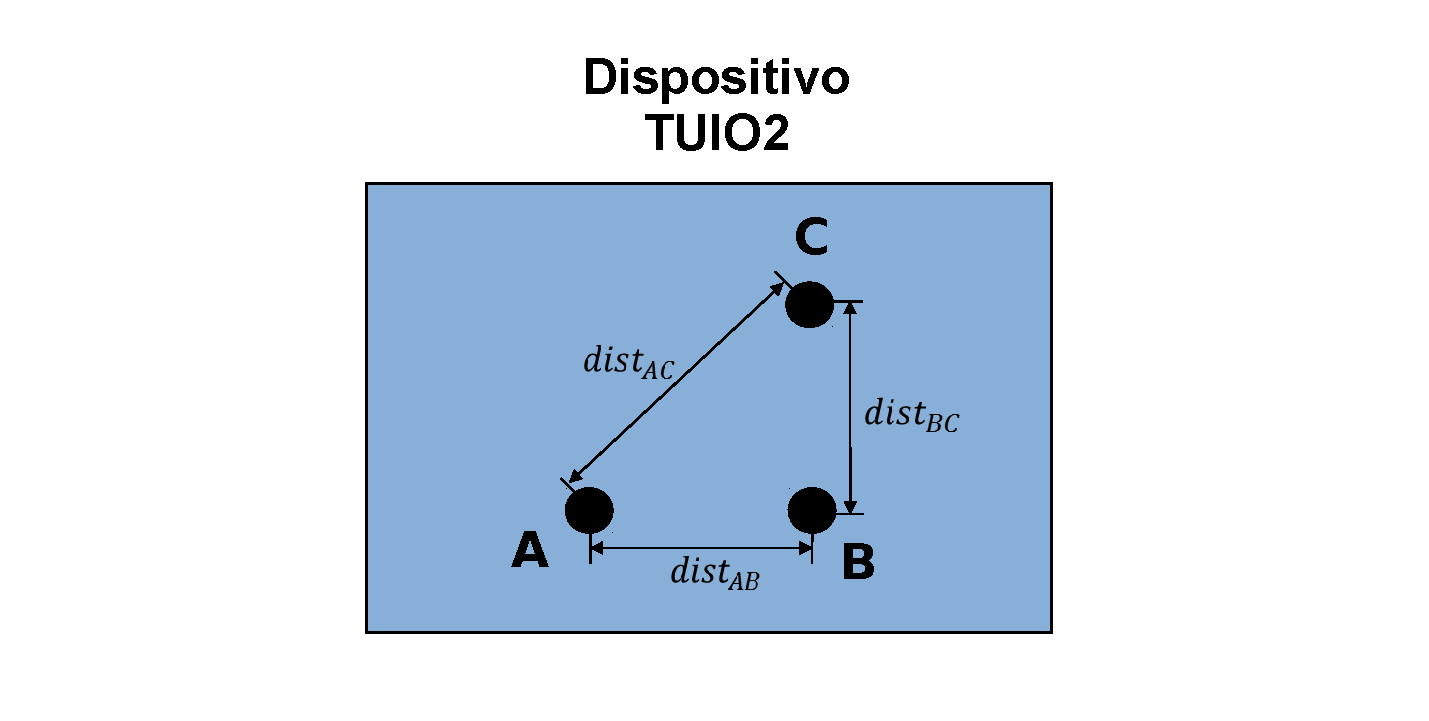
\includegraphics[width=0.9\textwidth]{localizacion3.pdf}
\caption{Versión de prueba no valida. Disposición de las almohadillas conductoras en la parte inferior del \emph{widget tangible} para generar los eventos táctiles. }
\label{fig:Localizacion3}
\end{center}
\end{figure}
Los tres puntos de contacto son identificados con las letras \textbf{A, B} y \textbf{C}, que dan nombre a los vértices de un triángulo rectángulo escaleno que forman. Se ha elegido este tipo de diseño, ya que cada uno de los tres lados tiene una medida diferente, lo que hace que sea más fácil identificar cada segmento del triángulo, y así evitar posibles problemas cuando se localice cualquiera de sus vértices.

Cuando \emph{TUIO2} está sobre la pantalla, los eventos táctiles generados, proporcionan la siguiente información al dispositivo \emph{TUIO1}: posición de las coordenadas (x,y), y número de evento. Las coordenadas de la posición de cada evento táctil está expresada en \emph{pixels}, por lo que cada evento producido será manejado en esas unidades de media (ver Figura~\ref{fig:Localizacion4}).\\
\begin{figure}[!h]
\begin{center}
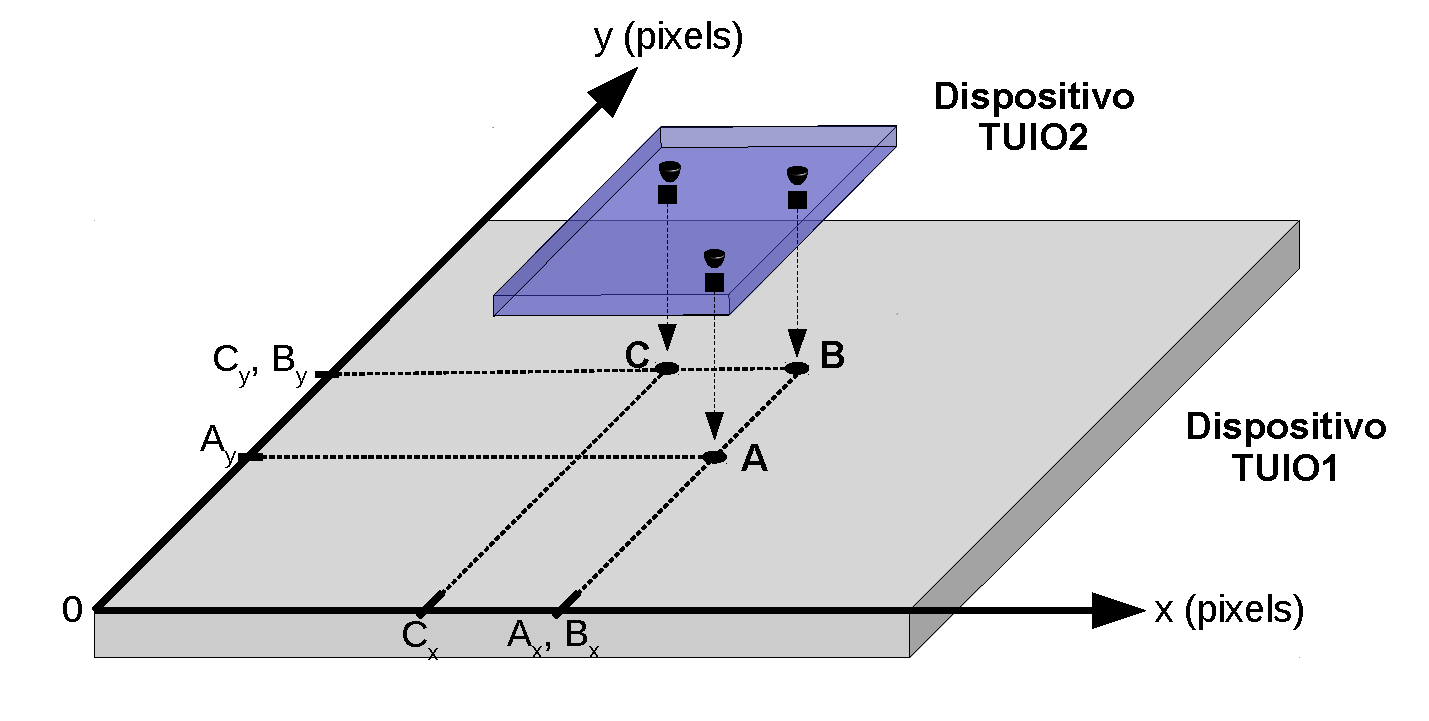
\includegraphics[width=0.9\textwidth]{localizacion4.pdf}
\caption{Versión de prueba no valida. Coordenadas de los puntos \textbf{A, B} y \textbf{C} del \emph{widget tangible} sobre la pantalla capacitiva. }
\label{fig:Localizacion4}
\end{center}
\end{figure}
Estos datos son interpretados y tratados para calcular la posición de \emph{TUIO2} en una librería desarrollada en \emph{Python}.

\subsubsection{Librería para la localización (Versión de prueba no valida).}

Todos los eventos táctiles generados sobre la pantalla capacitiva del dispositivo \emph{TUIO1}, son manejados por la \emph{clase Widget} de \emph{Kivy}, con el método \texttt{on\_touch\_down().}

Este método obtiene la información de posición e ID del evento táctil producido, almacenando estos datos en la lista \texttt{touch[].}

Se crea una librería específica para el manejo de esta lista, la cual tratará y manejara los datos para obtener la información de posición de \emph{TUIO2}.

\textbf{Método \texttt{pulsacion(touch)}} (Versión de prueba no valida).

El argumento de entrada, corresponde con las coordenadas y número de evento táctil, que contiene la lista de eventos (\texttt{touch}).\\
Estos datos son almacenados en la última posición de la lista \texttt{puls[]} aplicando el método \texttt{append()}:\\
\texttt{self.puls.append((t.x,t.y,t.id))}.\\
donde: \\
\texttt{t.x}: coordenada x del evento táctil.\\
\texttt{t.y}: coordenada y del evento táctil.\\
\texttt{t.id}: identificación del evento táctil (número de evento).

Cuando el número de eventos almacenados en \texttt{puls[]} 
es mayor que 1, se llama al método \texttt{determinar\_distancias()}.

\textbf{Método \texttt{determinar\_distancias()}} (Versión de prueba no valida).

El método \texttt{Vector()}, de la librería \texttt{kivy}, calcula la distancia entre los eventos táctiles producidos hasta el momento, que son almacenados en la lista \texttt{puls[]}. Estos eventos son recorridos desde el último elemento de la lista \texttt{puls[]}, hasta el primero. El método \texttt{determinar\_lados} determina las distancias entre puntos. Si la distancia es correcta, se incrementa la variable \texttt{contador}, la cual al llegar a 2, llama al método \texttt{determinar\_puntos()}.

\textbf{Método \texttt{determinar\_lados()}} (Versión de prueba no valida).

Método para verificar si dos eventos táctiles, cuyas distancias ya han sido determinadas, corresponden con uno de los lados del triángulo en el \emph{widget tangible}, donde \textit{m} corresponde con la distancia entre los dos eventos táctiles, \textit{i} el tamaño de la lista \texttt{puls[]}, y \texttt{a} el número de iteración del bucle que recorre cada uno de los elementos de la lista.

Este método es llamado cada vez que el método \texttt{determinar\_distancias()} es invocado.
Se comprueba si la distancia entre los dos puntos corresponde con el rango de medidas establecidas para los lados del triángulo del \emph{widget tangible}. Los rangos de medida se muestran en la tabla ~\ref{tab:intcor}.

\begin{table}[H]
\centering
{\small
\begin{tabular}{p{.2\textwidth}p{.2\textwidth}}
  \tabheadformat
  \tabhead{Rango}   &
  \tabhead{Segmento del triángulo}  \\
\hline
(120,150) & AB \\
\hline
(160,150) & BC \\
\hline
(210,260) & AC
\end{tabular}
}
\caption[Intervalos de medida de cada segmento del triángulo]{Intervalos de medida de cada segmento del triángulo}
\label{tab:intcor}
\end{table}

Si la medida corresponde con alguno de los rangos establecidos, dicha medida es almacenada junto con las coordenadas de ambos eventos en la lista \texttt{dist[]}. Por ejemplo, si la distancia entre los dos eventos táctiles es correcta, y corresponde al segmento \textbf{AB}, los datos son añadidos en la lista \texttt{dist[]}:

\texttt{self.dist.append((m,'AB',toq1,toq2)) }

donde \texttt{m} corresponde a la distancia entre ambos puntos, \texttt{AB} es el nombre del segmento al que corresponde, \texttt{toq1} son las coordenadas del evento táctil con el cual se está verificando la distancia en el método \texttt{determinar\_distancias()}, y \texttt{toq2} son las coordenadas del ultimo evento táctil.
Si la distancia es correcta se incrementa en una unidad la variable \texttt{contador}.

\textbf{Método \texttt{determinar\_puntos()}} (Versión de prueba no valida).

Este método es invocado dentro del método \texttt{determinar\_distancias()}, cuando la variable \texttt{contador} es mayor a 1, es decir, existen dos segmentos correctos del triángulo cuyos datos han sido almacenados en la lista \texttt{dist[]}, la cual contiene en ese momento dos elementos.
Los puntos del triángulo \textbf{(A,B,C)}, son calculados siguiendo la siguiente lógica:

Si los segmentos de los elementos de \texttt{dist[]} corresponden con $\overline{BC}$ y $\overline{AB}$ respectivamente, se llama al método \texttt{asignar\_puntos}, donde los argumentos de entrada se establecen:

\texttt{self.asignar\_puntos(1,2,0,'B','C','A')}

\textbf{Método \texttt{asignar\_puntos()}} (Versión de prueba no valida).

Este método asigna a cada vértice \textbf{A, B} y \textbf{C} del triángulo, las coordenadas donde se encuentran cada uno de ellos, al igual que el nombre del vértice. Estos datos son almacenados en la lista \texttt{coordenadas[]}

Para establecer un orden a la hora de añadir valores a la lista \texttt{coordenadas[]}, es pasado como argumento, la posición a la que corresponden cada uno de los puntos.

0: corresponde a la posición de la letra A en la lista \texttt{coordenadas[].}\\
1: posición de la letra B para la lista \texttt{coordenadas[]}.\\
2: posición de la letra C en la lista \texttt{coordenadas[]}.\\

La finalidad es que la lista \texttt{coordenadas} quede con la siguiente estructura, para ser manejada:\\

$[(x_{A},y_{A},'A'),(x_{B},y_{B},'B'),(x_{C},y_{C},'C')]$\\

En el ejemplo anterior, los elementos de \texttt{dist[]} corresponden con $\overline{BC}$ y $\overline{AB}$. El punto en común para ambos segmentos corresponde a \textbf{B}, \textbf{C} para el primer segmento, y \textbf{A} para el segundo segmento.

El método para asignar los puntos es:

\texttt{self.asignar\_puntos(1,2,0,'B','C','A')}\\
donde los argumentos de entrada son:
c = 1, posición del punto en común entre los dos segmentos. Como el punto en común es \textit{B} que corresponde con la posición 1 de la lista \texttt{coordenadas[]}.\\
c1 = 2, es la posición del punto \textbf{C} para el ejemplo según el criterio establecido.\\
c2 = 0, corresponde a la posición del punto \textbf{A} para la lista \texttt{coordenadas[]}.\\
p = 'B', Nombre del vértice en común, en este ejemplo corresponde al vértice \textbf{B}.\\
p1 = 'C', Nombre del vértice restante del primer segmento, en este caso el primer segmento es el $\overline{BC}$, por lo tanto, el vértice corresponde al \textbf{C}.\\
p2 = 'A', Nombre del vértice del segundo segmento, que corresponde con el vértice \textit{A}.\\

Los valores que contiene la lista \texttt{dist[]} para ser manejados por el método \texttt{asignar\_puntos()} son:
\texttt{[(0, 'NADA'), (164.0, 'BC', (440.00000000000006, 346.0, 'mouse2'), (440.00000000000006, 182.0, 'mouse1')), (134.03357788255903, 'AB', (306.0, 179.0, 'mouse3'), (440.00000000000006, 182.0, 'mouse1'))]}\\

La lista es recorrida mediante el siguiente bucle (ver Listado~\ref{code:buclevertices}):
\begin{lstlisting}[
float = ht, 
language = python,
caption = {Bucle para asignar las coordenadas de los vértices (Versión de prueba no valida).},
label = code:buclevertices]
for a in r
	for b in range(2):
		if self.dist[1][a+2][2] == self.dist[2][b+2][2]:
			self.coordenadas[c] = (self.dist[1][a+2][0],self.dist[1][a+2][1],p)
			if a == 0:
				self.coordenadas[c1] = (self.dist[1][3][0],self.dist[1][3][1],p1)
			else:
				self.coordenadas[c1] = (self.dist[1][2][0],self.dist[1][2][1],p1)
			if b == 0:
				self.coordenadas[c2] = (self.dist[2][3][0],self.dist[2][3][1],p2)
			else:
				self.coordenadas[c2] = (self.dist[2][2][0],self.dist[2][2][1],p2)
			break
\end{lstlisting}

Donde \texttt{a} es la posición para el primer elemento de la lista \texttt{dist[]}, y \texttt{b} la posición del segundo elemento de la lista.

Para poder analizar mejor este ejemplo, separamos los dos elementos de la lista \texttt{dist[]}:

\texttt{Elemento 1 de dist[]}:

\texttt{(164.0, 'BC', (440.00000000000006, 346.0, 'mouse2'), (440.00000000000006, 182.0, 'mouse1'))}

\texttt{Elemento 2 de dist[]}:

\texttt{(134.03357788255903, 'AB', (306.0, 179.0, 'mouse3'), (440.00000000000006, 182.0, 'mouse1'))}

La \textit{posición 0} corresponde a la distancia entre segmentos, la \textit{posición 1} es el nombre del segmento, y las dos restantes posiciones son las coordenadas de los puntos del segmento junto con la \textit{id} del evento táctil.\\

\texttt{id: 'mouse1'} es el elemento en común para los dos segmentos, en este caso $\overline{BC}$ y $\overline{AB}$, donde el punto en común es el punto \textit{B}. Por lo tanto:\\

\texttt{self.coordenadas[c] = (self.dist[1][a+2][0],self.dist[1][a+2][1],p)}\\

Las coordenadas del punto \textbf{B} (coordenada x y coordenada y) son almacenadas en la lista \texttt{coordenadas[]}, al igual que el nombre del vértice común (argumento \texttt{p = 'B'}), en la posición \texttt{c}, que como argumento de entrada se indicó como 1 (punto \textbf{B}). 

La posición de \texttt{'mouse1'} para el primer elemento de \texttt{dist[]}, es para un valor de \texttt{a} igual a 1 (ya que al valor de \texttt{a}, se le suma 2 posiciones, por ser los dos primeras, la distancia entre segmentos, y el nombre del segmento), es decir, la posición 3 del elemento 1 de \texttt{dist[]}.

Para el segundo elemento, la posición del vértice \textit{B} corresponde a un valor de \texttt{b = 1} como en el caso del primer segmento.
Una vez asignada las coordenadas del punto en común, el nombre del vértice, y almacenados dichos datos en la lista \texttt{coordenadas[]} en la posición 1, son determinadas las coordenadas de los dos puntos restantes del triángulo (\textbf{C} y \textbf{A}): 
Con los tres vértices del triángulo, se calcula el área del triángulo mediante la llamada al método \texttt{calculo\_area}, para verificar que el triángulo es correcto y corresponde con las posiciones del \emph{widget tangible} y no responde a un error de eventos sobre la pantalla táctil.

\textbf{Método \texttt{calculo\_area()}} (Versión de prueba no valida).
El método \texttt{calculo\_area}, retorna el valor del área, la cual, se debe encontrar en el intervalo (9545,16000). 
Si el área no es correcta, se realiza una llamada al método \texttt{inicializar\_a\_0}, para restablecer los valores a sus condiciones iniciales. 

Se aplica la \emph{regla de Sarrus} (determinante), para el cálculo del área. El argumento de estrada es la lista \texttt{coordenadas[]} que contiene las coordenadas de los vértices del triángulo:

\texttt{det = abs((c[0][0]*c[1][1])+(c[0][1]*c[2][0])+(c[2][1]*c[1][0])}\\
\texttt{-((c[1][1]*c[2][0])+(c[0][1]*c[1][0])+(c[0][0]*c[2][1])))*0.5}.\\



\subsubsection{Validación de la librería para el sistema de localización.}

Las pruebas realizadas siguiendo el patrón de un triángulo equilátero escaleno, arrojan fallos significativos durante el proceso del cálculo de las coordenadas y ángulo de posición, del dispositivo \emph{TUIO2}, destacando los siguientes problemas:
\begin{itemize}
\item Determinación incorrecta de los vértices en distintas etapas de la localización.
\item La adquisición de datos queda en estado de espera, cuando son detectados eventos táctiles involuntarios sobre el sensor capacitivo.
\item Medidas erróneas captadas por el sensor capacitivo, debidas a la poca estabilidad de los puntos de contacto de las almohadillas conductoras, retornando valores inexactos de posición.
\item Poca organización del código y del tratamiento de datos.
\end{itemize}

Todos estos resultados obligan a determinar un nuevo patrón de localización, al igual que simplificar los procedimientos de almacenamiento y procesado de datos.
 
\subsection{Versión de pruebas 2. Localización de coordenadas con patrón lineal.}

Esta versión de pruebas del sistema de localización tiene como objetivo optimizar los procesos de adquisición y tratamiento de datos, aplicando diferentes patrones para determinar la posición y ángulo del dispositivo \emph{TUIO2}.

La situación de las almohadillas conductoras ha sido modificada, aplicando un patrón de tres puntos \textbf{(0, A, B)} situados en paralelo a la parte inferior del dispositivo, tomando como puntos de referencia, la esquina posterior izquierda \textbf{(0)}, y posterior derecha\textbf{(B)}. El tercer punto queda situado a una distancia de \textbf{(0-A) > (A-B)} (ver Figura~\ref{fig:coorlineal}). Tomando como referencia un vector, el punto B determinaría la dirección de dicho vector.

\begin{figure}[!h]
\begin{center}
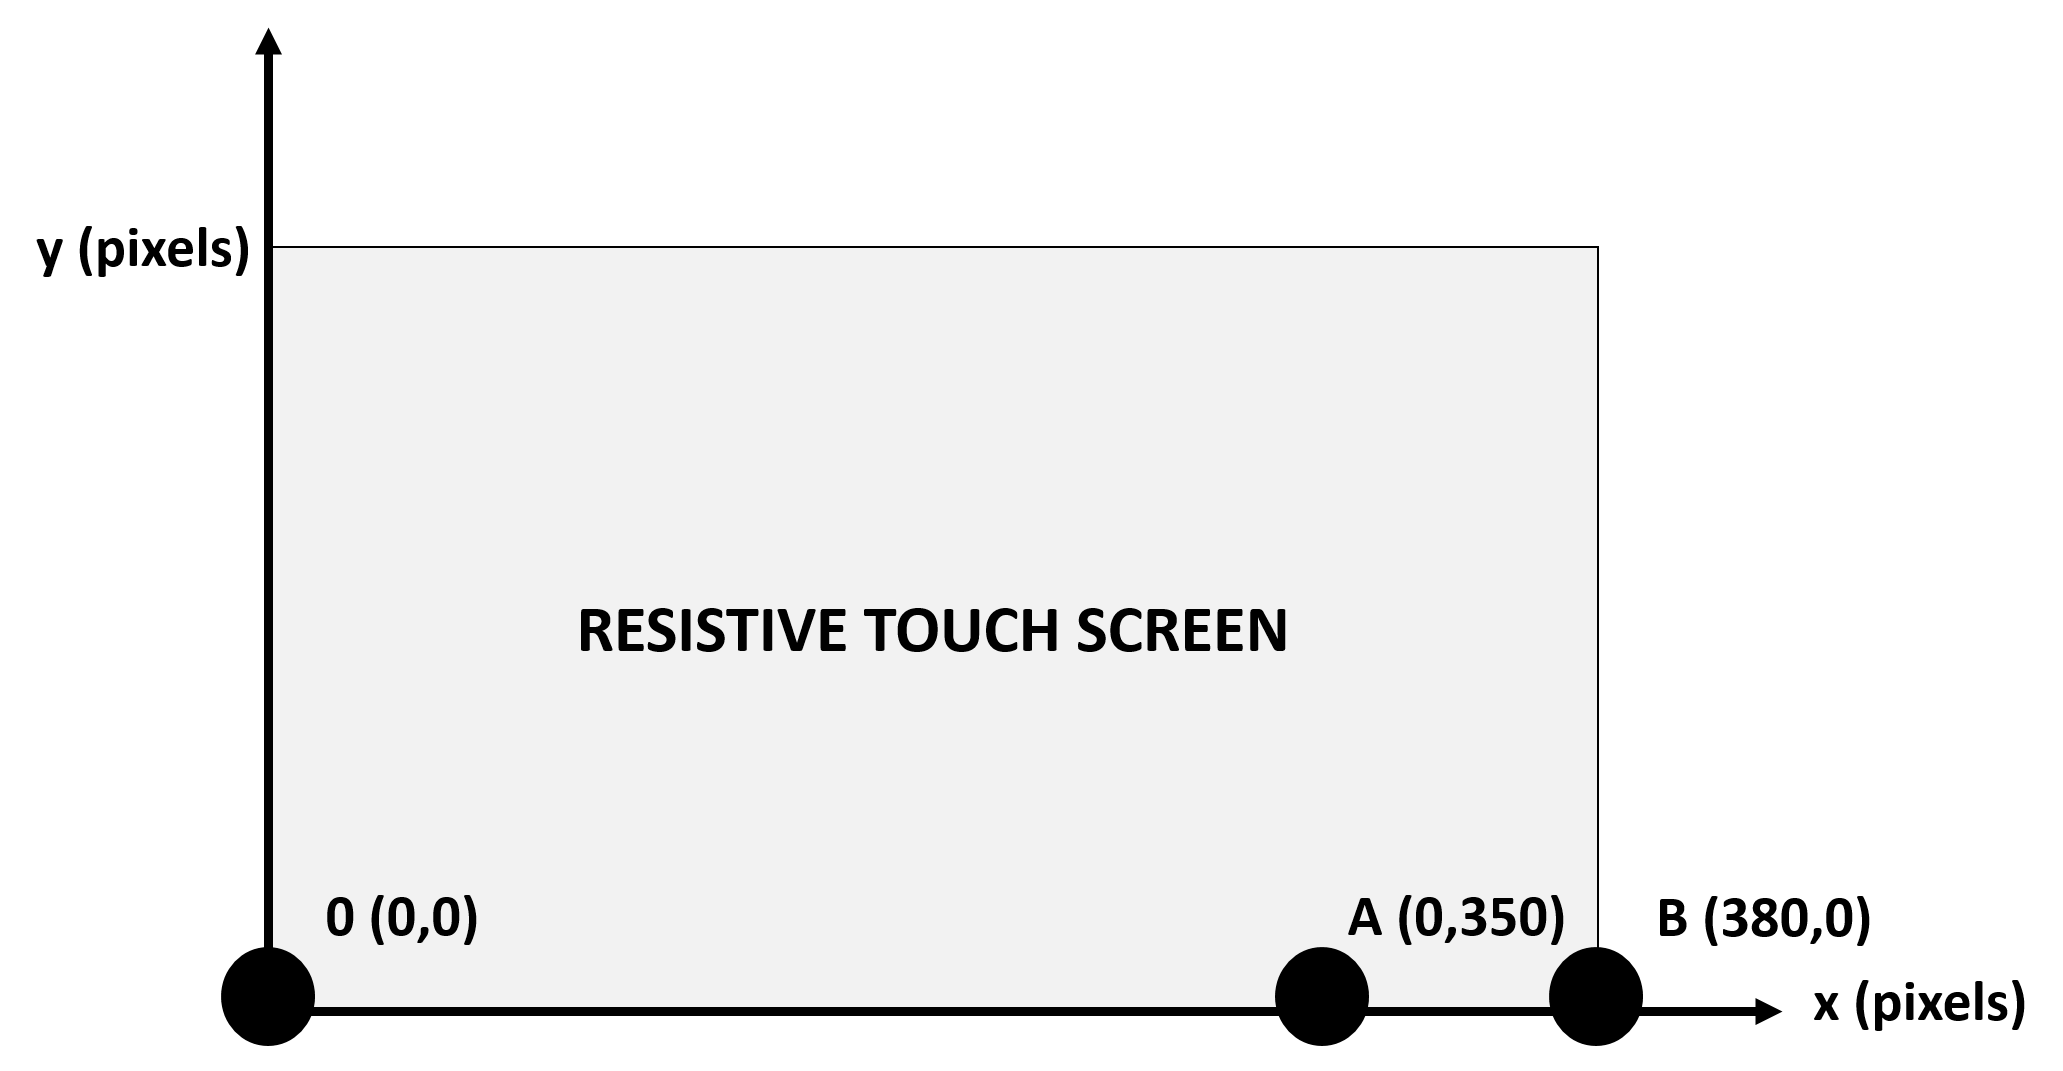
\includegraphics[width=0.9\textwidth]{coordenadas_almohadillas.png}
\caption{Situación de los puntos \textbf{A, B} y \textbf{C} del \emph{widget tangible} en \emph{TUIO2}. }
\label{fig:coorlineal}
\end{center}
\end{figure}

El procedimiento de calculo obtiene las coordenadas del punto 0, que corresponde con el origen de coordenadas de las representaciones gráficas en \emph{TUIO2}.
La adquisición de la posición y ángulo del dispositivo tiene la siguiente finalidad:
\begin{itemize}
\item Punto de referencia 0: trasladar la representación gráfica del dispositivo \emph{TUO2}, acorde con la representación gráfica de \emph{TUIO1} al ser situado sobre el sensor capacitivo.
\item Ángulo de inclinación: obtener una correcta representación gráfica en \emph{TUIO2}, al ser posicionado con un ángulo de inclinación con respecto al sistema de coordenadas de la representación gráfica de \emph{TUIO1}.
\end{itemize}
Estos datos, junto con un escalado correcto de los elementos gráficos en \emph{TUIO2}, permite obtener de manera correcta, los elementos situados bajo el dispositivo al ser detectado por el sensor capacitivo (Figura~\ref{fig:touchcoord}).

\begin{figure}[!h]
\begin{center}
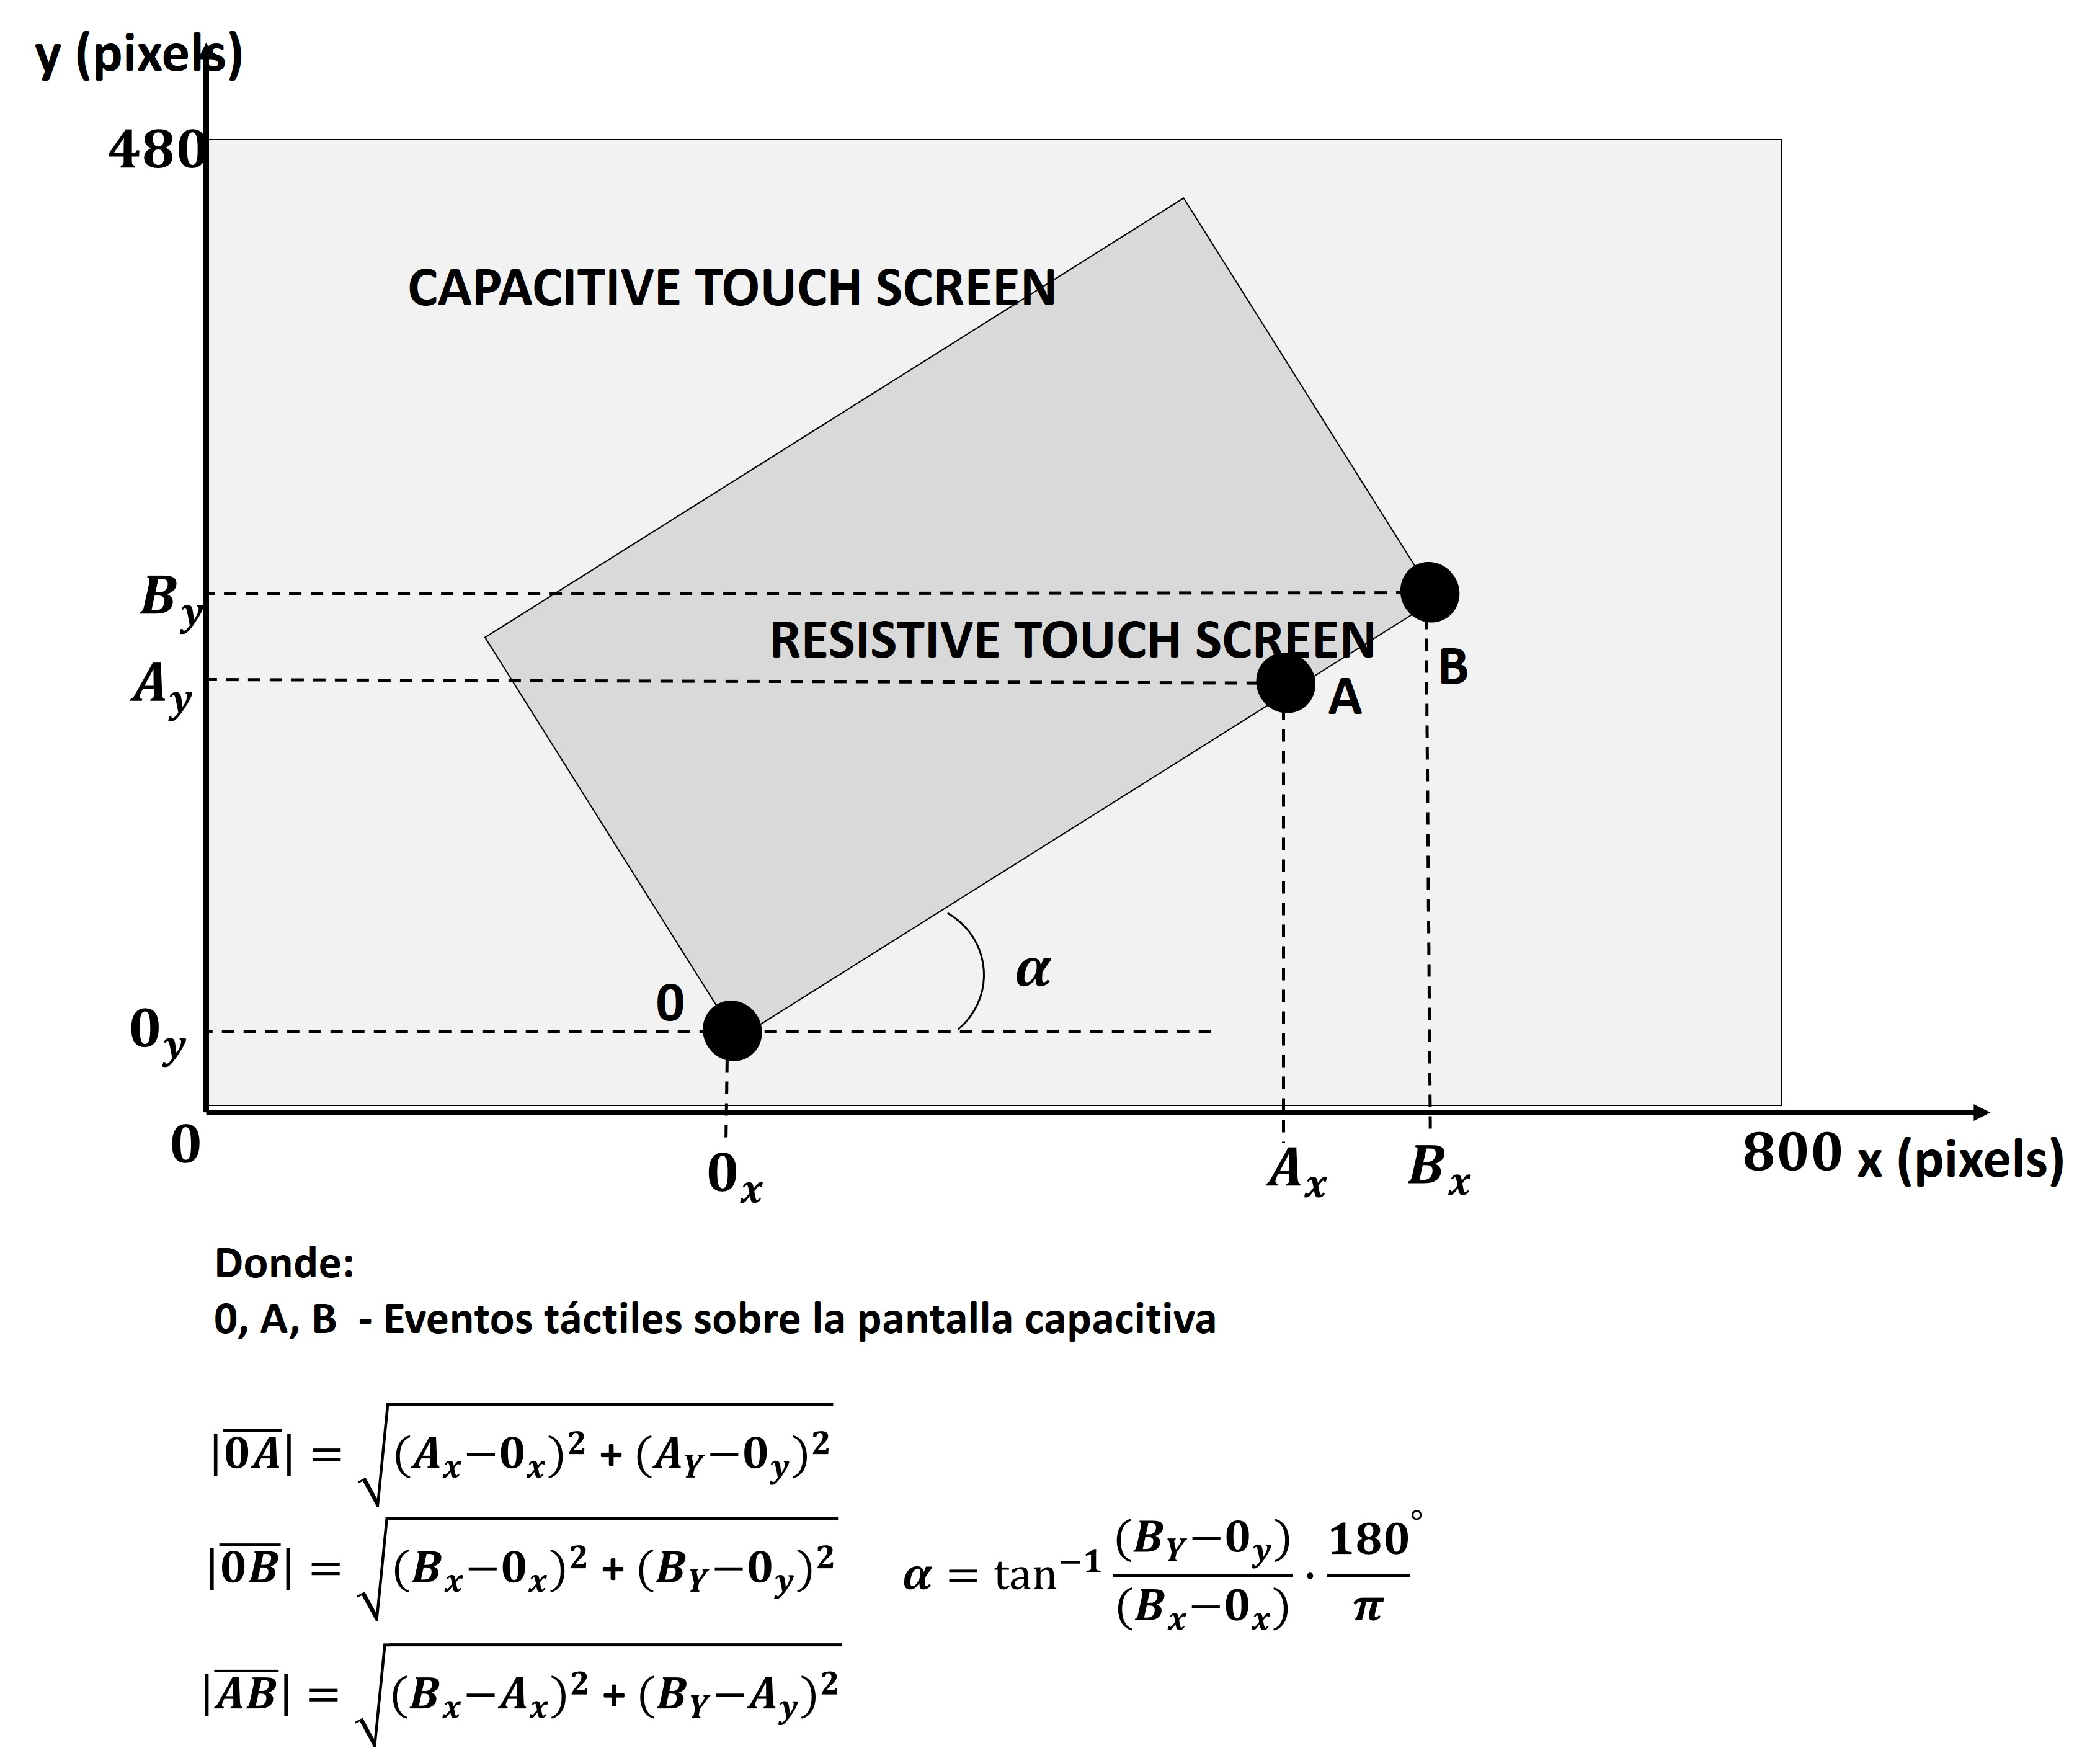
\includegraphics[width=0.9\textwidth]{touch_coordinates.jpg}
\caption{Situación de los puntos \textbf{A, B} y \textbf{C} del \emph{widget tangible} en \emph{TUIO2}, sobre la pantalla táctil capacitiva del dispositivo \emph{TUIO1} }
\label{fig:touchcoord}
\end{center}
\end{figure}

\subsubsection{Librería para la localización.}
El módulo desarrollado para la localización se divide en dos clases.
Clase para la obtención de eventos táctiles: \texttt{TouchInput}.
Clase para el cálculo del ángulo y punto de referencia. \texttt{TouchPositions}.

\textbf{Clase \texttt{TouchInput}.}\\ 
Clase que hereda de la clase \texttt{Widget} del módulo \texttt{kivy.uix.widget}. Esta clase obtiene los eventos táctiles producidos sobre la pantalla de manera automática. Se crea el objeto \texttt{touch\_positions} de la Clase \texttt{TouchPosition}, para realizar los cálculos a partir de los eventos producidos.

Métodos de clase.
\begin{itemize}
\item \texttt{on\_touch\_down()}: el atributo \texttt{touch} indica la posición y número de toque del evento táctil. El evento es registrado en el \emph{diccionario} \texttt{touchs}, del objeto \texttt{touchs\_positions}.

\item \texttt{on\_touch\_up()}: obtiene los datos de posición y número de evento táctil, al ser desacoplado. El número de evento es utilizado para ser eliminado del diccionario de eventos táctiles \texttt{touchs}.
\end{itemize}
\textbf{Clase \texttt{TouchPositions}.}\\ 
Esta clase hereda de la clase base \texttt{object}, y contiene los métodos para el calculo de las posiciones de los puntos de contacto de los eventos táctiles.

Métodos de clase.
\begin{itemize}
\item \texttt{add\_touch()}. Añade los eventos táctiles en el diccionario \texttt{touch}, tomando como clave el número de evento táctil.

\item \texttt{remove\_touch()}: Elimina los eventos táctiles que han sido desacoplados, utilizando la clave del evento táctil sobre el diccionario de datos \texttt{touch}.

\item \texttt{calculate\_distance()}: Calcula la distancia entre dos eventos táctiles, utilizando el método \texttt{Vector} de la clase \texttt{Vector} del módulo \texttt{kivy.vector}. Llamada al método \texttt{calculate\_segments} para verificar si la distancia corresponde con el patrón predefinido. La distancia es guardada de manera temporal en la variable local \texttt{dist}.

\item \texttt{calculate\_segments()}: Determina si la distancia corresponde con los márgenes del patrón de localización. Si el segmento es correcto, se almacenan las coordenadas de los puntos del segmento en un diccionario de datos, con las tres claves posibles \texttt{(0A), (0B), (AB)}.

\item \texttt{calculate\_points()}: Obtiene la correspondencia de los puntos \textbf{0, A, B}, con las coordenadas de los eventos táctiles. Las coordenadas son almacenadas en tres variables locales, para ser usadas como argumento de entrada en el método \texttt{calculate\_angle}.

\item \texttt{calculate\_angle()}: Las coordenadas del punto de referencia \textbf{0} y las coordenadas el punto \textbf{A/B}, se calcula el ángulo del sistema de coordenadas de \emph{TUIO2}, con respecto al sistema de coordenadas de \emph{TUIO1}, con la función \texttt{atan2} de la librería \texttt{math}.
\end{itemize}
Los datos de las coordenadas del punto de referencia \textbf{0} de \emph{TUIO2}, y el ángulo, son almacenados en la cola de eventos \texttt{events}.

\subsubsection{Validación de la librería para el sistema de localización.}
Las pruebas de localización realizadas con un patrón lineal arrojan ciertas mejorías sobre el patrón triangular aplicado en la primera versión de pruebas, destacando los siguientes aspectos:
\begin{itemize}
\item Determinación correcta de los puntos de coordenadas \textbf{A,B,C} correspondientes al patrón lineal.
\item Mejora en el cálculo del ángulo del sistema de coordenadas de \emph{TUIO2} con respecto a \emph{TUIO1}. 
\end{itemize}
Las variaciones en el ángulo se deben principalmente a errores del sensor capacitivo, con los puntos de contacto de las almohadillas conductoras.

\section{Diseño software de la interfaz gráfica.}

\subsection{Manejo de eventos de la interfaz.}

Todos los eventos relacionados con cambios producidos en las representaciones gráficas en la plataforma de juego, son gestionados con los métodos de la clase \texttt{InterfaceManagement}, y el objeto de clase \texttt{ScreenManager}.

\texttt{InterfaceManagement} maneja los eventos de entrada desde el módulo principal \texttt{Tuio1FSM/Tuio2FSM}, y los eventos táctiles procedentes desde la propia interfaz gráfica de usuario.

\texttt{ScreenManager} gestiona los eventos de entrada desde los módulos dedicados a juegos, principalmente para realizar cambios de pantalla (\texttt{Screen}).

\textbf{Instancia del objeto \texttt{screenmanager}.}

El objeto \texttt{screenmanager} es instanciado de manera global, para facilitar el manejo de eventos gráficos por el resto de los módulos de la aplicación, ya que los juegos disponen de sus propias pantallas (\texttt{Screens}), y sus propios objetos gráficos, que son añadidos a las mismas.

La estructura del manejo y gestión de eventos sigue una distribución secuencial, como se muestra en la Figura~\ref{fig:interfacevent}).

\begin{figure}[!h]
\begin{center}
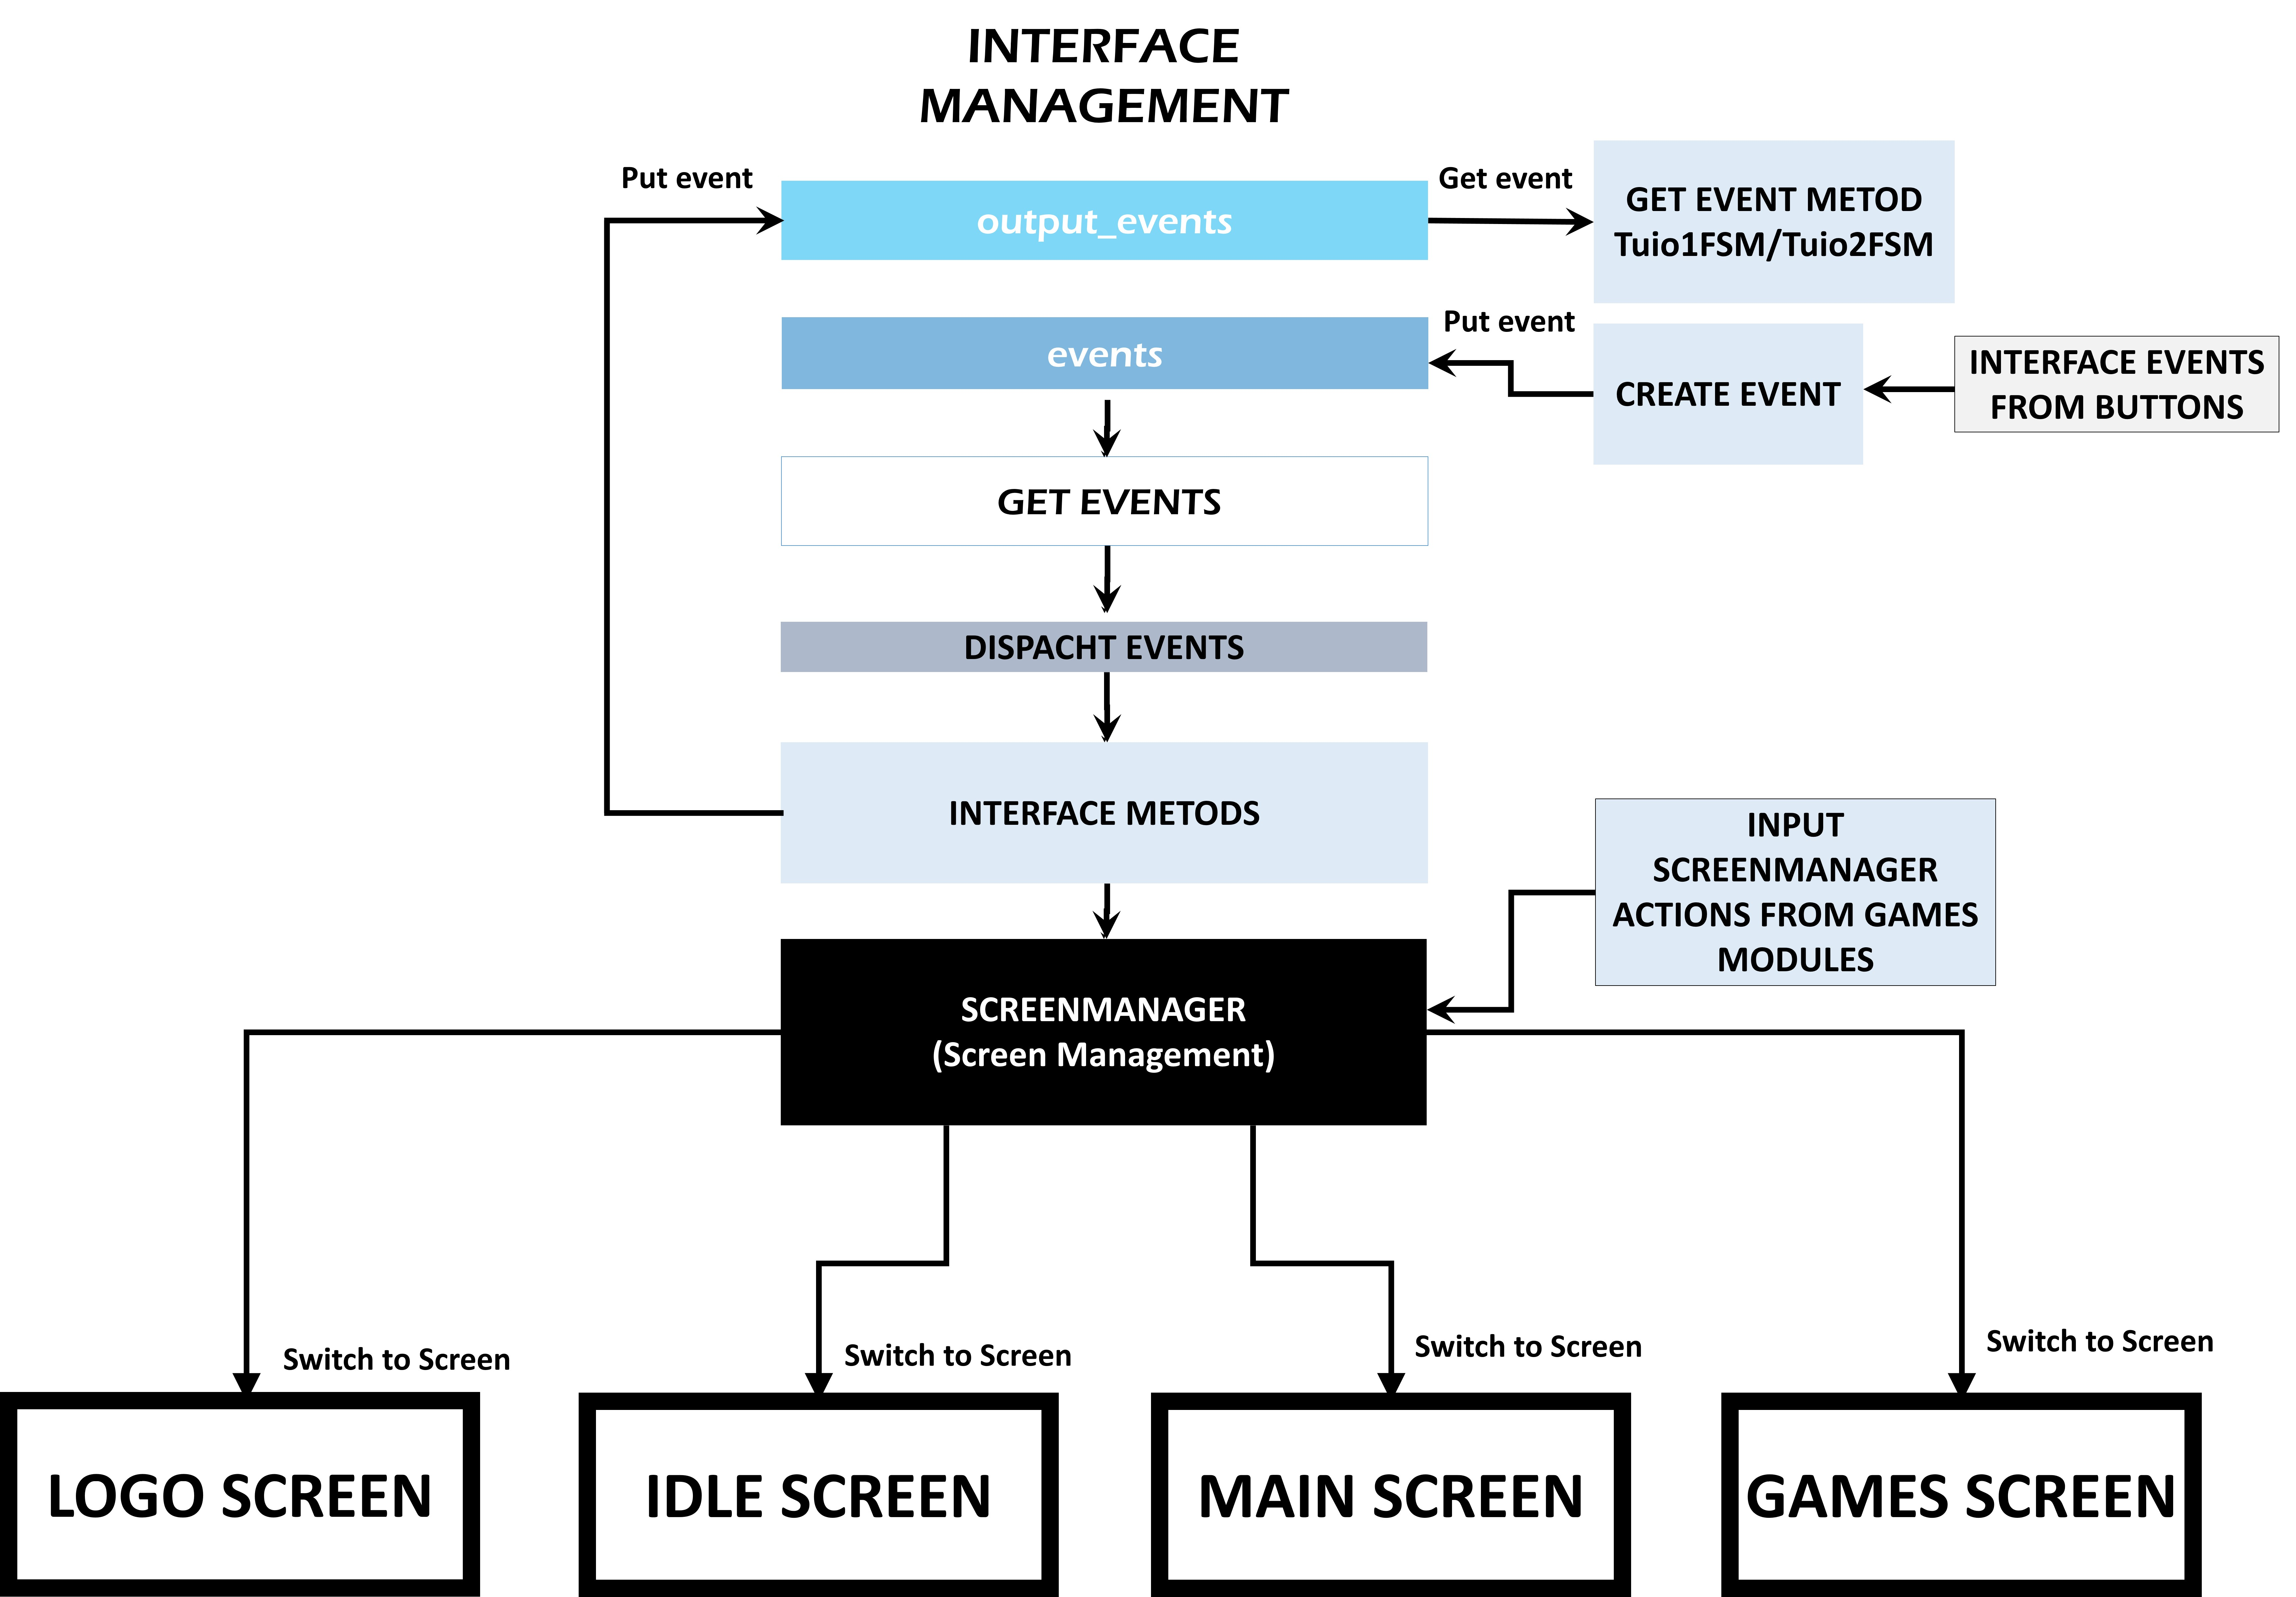
\includegraphics[width=0.9\textwidth]{interface_events.jpg}
\caption{Estructura de la gestión de eventos del módulo \texttt{InterfaceManagement()}.}
\label{fig:interfacevent}
\end{center}
\end{figure}


\subsection{Módulo para el manejo de la interfaz \texttt{InterfaceManagement}.}

\textbf{Módulos \texttt{ScreenManager} y \texttt{Screen}.}

\texttt{ScreenManager} y \texttt{Screen}, son módulos del paquete \texttt{uix} de la librería \texttt{Kivy}, que disponen de los métodos de clase básicos para el diseño, y manejo de eventos gráficos generados durante el transcurso de la aplicación. 

\texttt{ScreenManager} es un \emph{widget} dedicado a administrar múltiples pantallas en la aplicación. Muestra solo una pantalla (\texttt{Screen}) a la vez, y usa la librería \texttt{TransitionBase} para cambiar de una pantalla a otra. 

\texttt{Screen} es un objeto destinado a ser utilizado con \texttt{ScreenManager}, donde son incorporados los diferentes elementos que componen la interfaz gráfica de usuario.

\subsubsection{Funcionamiento básico de \texttt{ScreenManager}.}

Importar módulos: \texttt{from kivy.uix.screenmanager import ScreenManager , Screen}

Crear el objeto \texttt{sm} (\emph{ScreenManager}): \texttt{sm = ScreenManager()}

Crear una pantalla: \texttt{screen = Screen(name='screen\_1')}

Añadir una pantalla al administrador: \texttt{sm.add\_widget(screen)}

Cambiar a la pantalla \texttt{'screen\_1'}: \texttt{sm.current = 'screen\_1'}


\subsubsection{Clases de la interfaz gráfica.}

\textbf{Clase \texttt{Widget()}}. Clase base requerida para crear \emph{widgets}.

Método de importación del módulo: \texttt{from kivy.uix.widget import Widget} //

\textbf{Clase \texttt{Button()}.} \texttt{Button} es una clase del módulo \texttt{Label}, que dispone de acciones asociadas, que son ejecutadas al ser presionado el botón, o cuando se deja de presionar. //

Método de importación del módulo: \texttt{from kivy.uix.button import Button}


\subsubsection{Pantallas (\texttt{Screens}), manejadas por los gestores de eventos \texttt{Tuio1FSM/Tuio2FSM}.}

\begin{itemize}
\item \textbf{Pantalla Logo. \texttt{LogoScreen}}.
Pantalla de bienvenida, que ejecuta una pequeña animación del nombre de la plataforma, al iniciar la aplicación.
\item \textbf{Pantalla Idle. \texttt{IdleScreen}.}
Pantalla que muestra una imagen (fondo de pantalla), indicando que la conexión no ha sido establecida. Se mantiene en ese estado hasta ejecutar el método de cambio de pantalla desde el gestor de eventos principal.
\item \textbf{Pantalla Main. \texttt{MainScreen}.}
Pantalla principal de la aplicación, una vez son establecidas las comunicaciones entre ambos dispositivos.
\end{itemize}


Métodos de clase para el manejo de la interfaz, con el módulo \texttt{InterfazManagement} \ref{tab:metointer}:
\begin{table}[H]
\centering
{\small
\begin{tabular}{p{.3\textwidth}p{.6\textwidth}}
  \tabheadformat
  \tabhead{Método}   &
  \tabhead{Descripción}  \\
\hline
\texttt{init\_interface()} & Inicio de la interfaz gráfica. Cambio a la pantalla \texttt{'logo\_screen'} (pantalla de bienvenida).  \\
\hline
\texttt{create\_event()} & Añade a la cola de eventos con el método \texttt{put()}, el argumento de entrada al método. \\
\hline
\texttt{get\_event()} & Obtiene el evento de la cola de eventos, con el método \texttt{get()}. \\
\hline
\texttt{dipatch\_event()} & Según el tipo de evento, se ejecutan los métodos de clase. \\
\hline
\texttt{main\_state()} & Ejecuta un cambio a la pantalla \texttt{'main\_screen'} con \texttt{ScreenManager}. \\
\hline
\texttt{idle\_state()} & Ejecuta un cambio a la pantalla \texttt{'idle\_screen'} con \texttt{ScreenManager}. \\
\hline
\texttt{close\_interface()} & Termina todos los procesos de la interfaz y de la aplicación, con el método texttt{stop()} de la clase \texttt{App}. \\
\end{tabular}
}
\caption[Métodos de la clase \texttt{InterfaceManagement()}]{Métodos de la clase \texttt{InterfaceManagement()}}
\label{tab:metointer}
\end{table}



\section{Lectura y configuración de sensores.}


\subsection{Unidad de medición inercial MPU-9255.}
La unidad de medición inercial integrada en la plataforma, es el sensor \emph{MPU9255}. Este sensor forma parte del dispositivo \emph{TUIO2}. Esta destinado principalmente a capturar eventos de movimiento, para generar acciones durante el transcurso del juego. Al realizar movimientos angulares sobre los ejes X,Y,Z del dispositivo \emph{TUIO2}, se generan unos eventos que son filtrados y comunicados al dispositivo \emph{TUIO1}, para ser ejecutados durante el transcurso del juego. Por ejemplo, girar una pieza representada en \emph{TUIO1}

\subsubsection{Conexionado Bus I2C MPU-9255.}


La conexión con la placa para el desarrollo \emph{Raspberry Pi} para comunicaciones \emph{I2C}, se realiza mediante 4 líneas (ver Figura~\ref{fig:MPU9255_I2C}).

\begin{figure}[!h]
\begin{center}
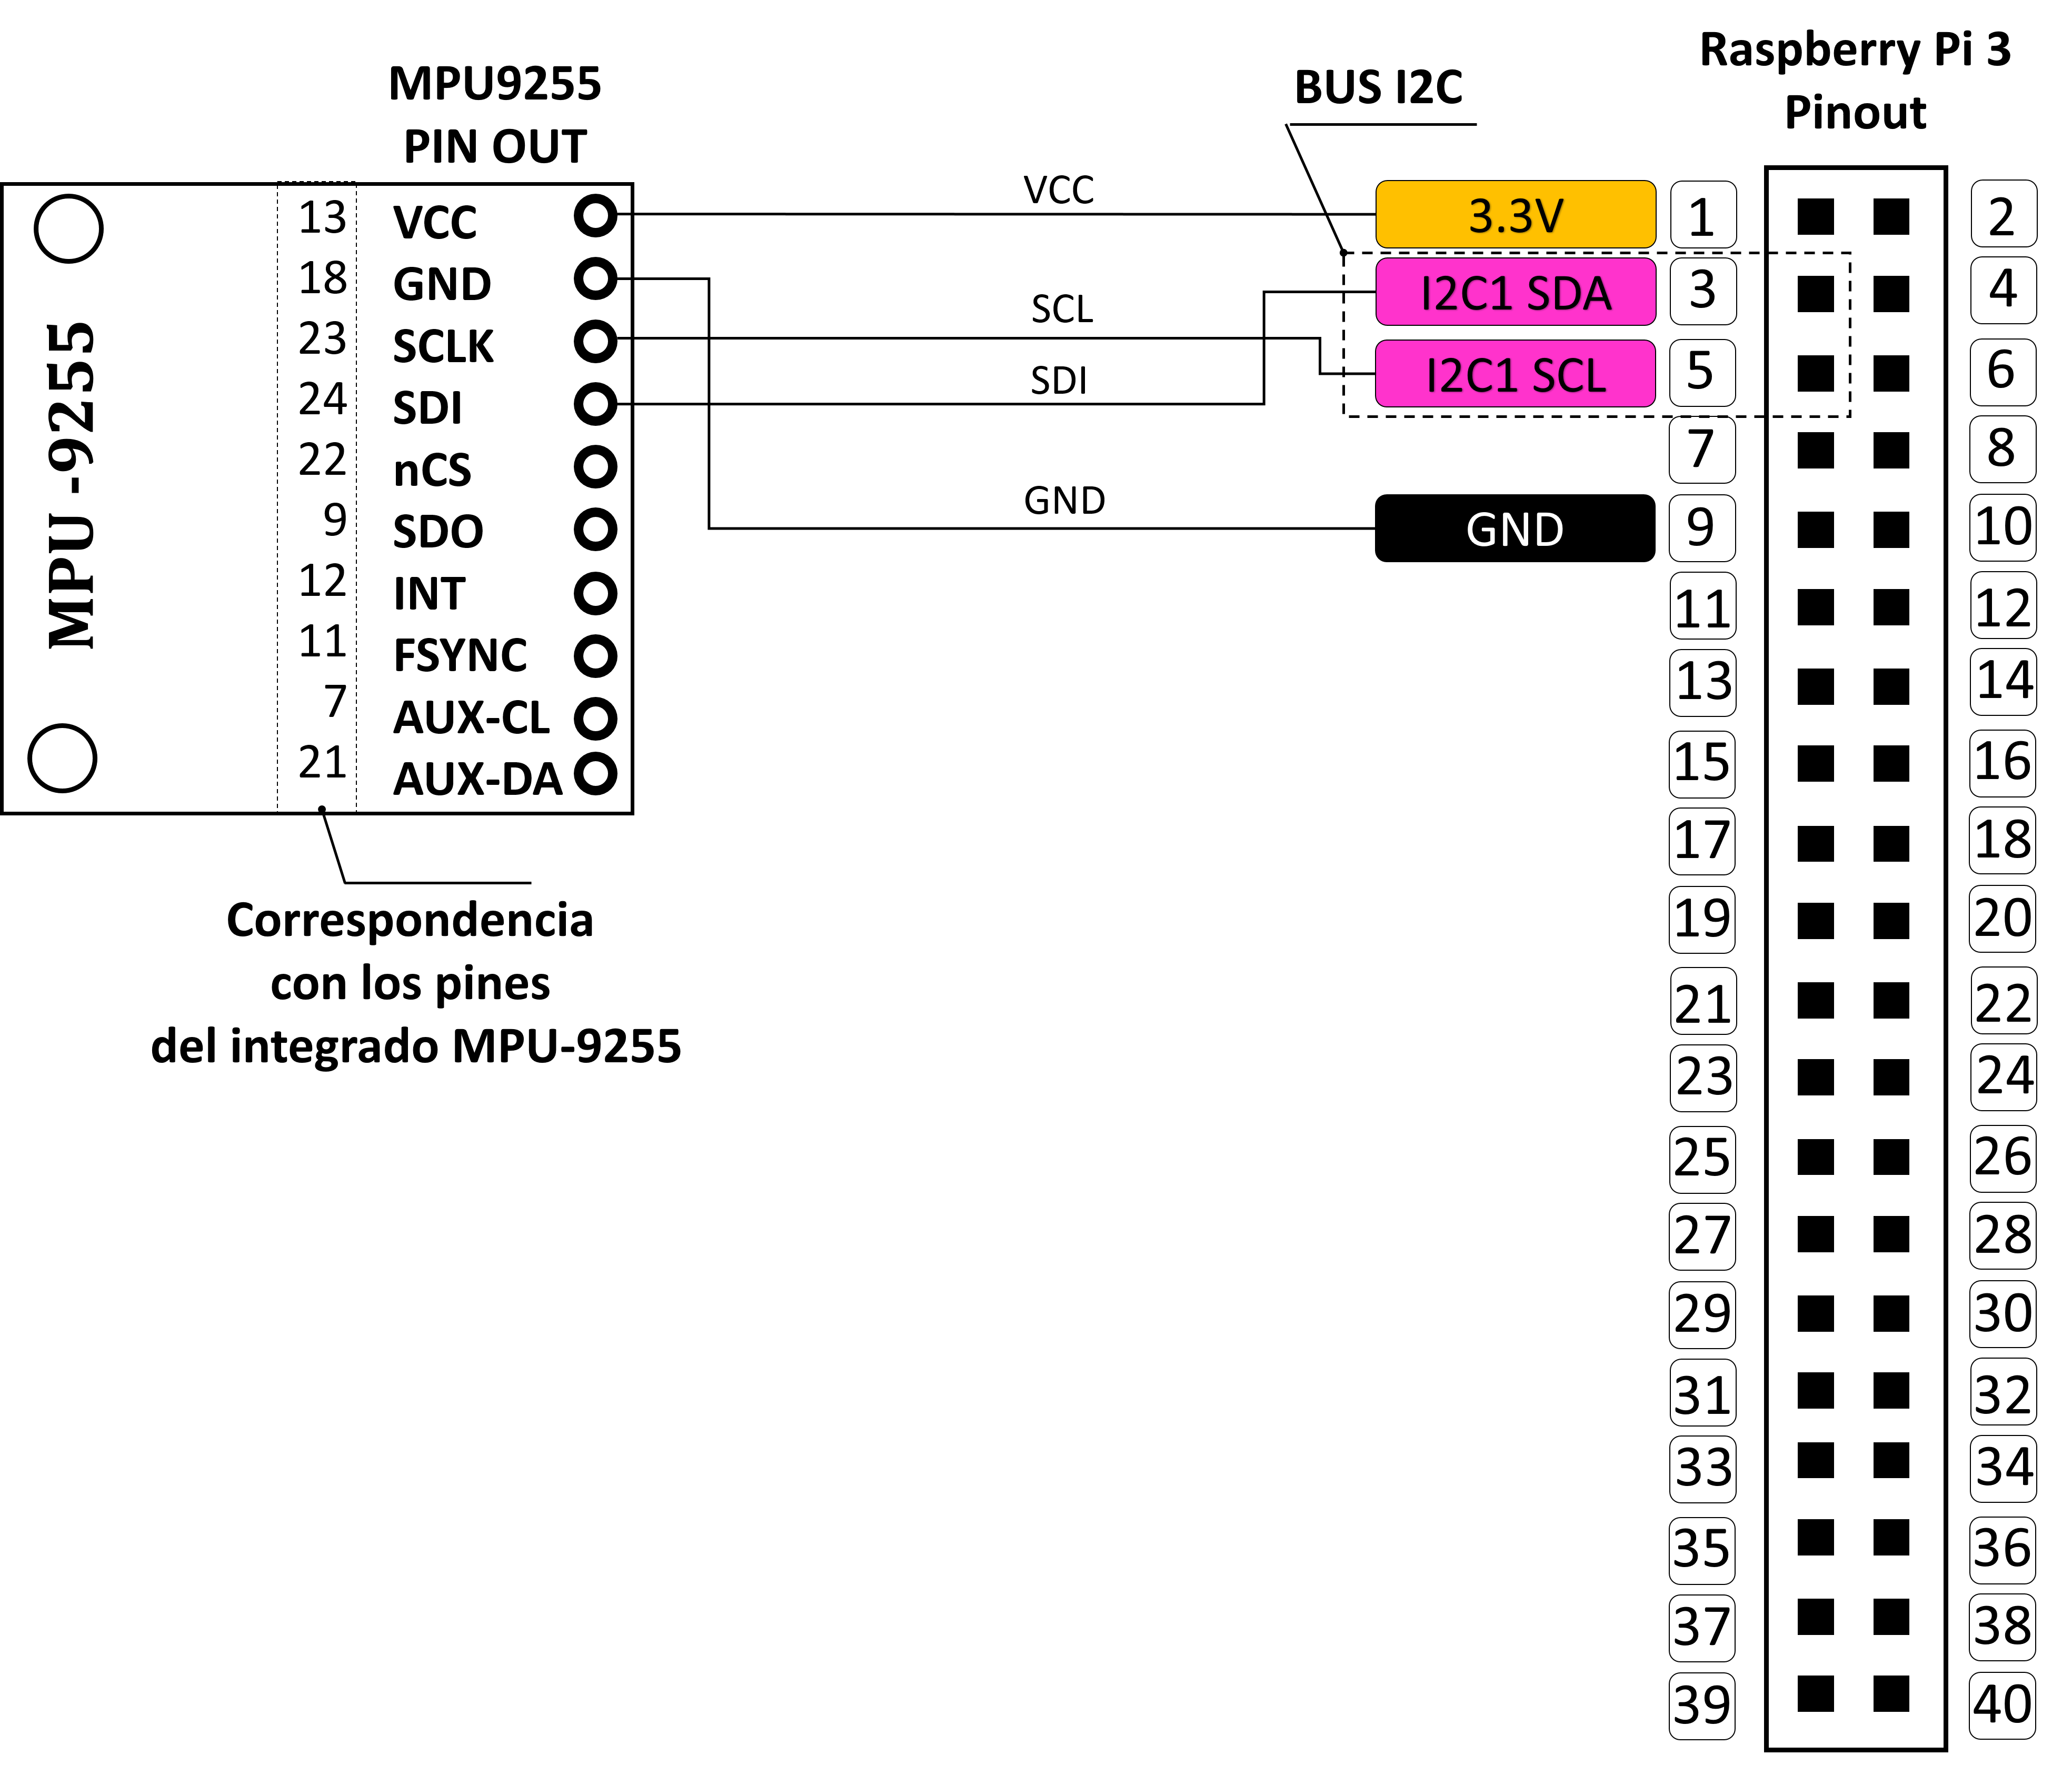
\includegraphics[width=0.8\textwidth]{MPU9255_PINOUT.png}
\caption{Esquema de conexiones con Raspberry Pi para comunicaciones I2C.}
\label{fig:MPU9255_PINOUT}
\end{center}
\end{figure}


\subsubsection{Configuración y lectura, de las posiciones de memoria MPU-9255.}

Para establecer comunicaciones mediante \emph{Bus I2C}, entre \emph{Raspberry Pi} y el \emph{sensor MPU-9255}, es necesario importar la librería: \texttt{smbus}

Las comunicaciones con el \emph{Bus I2C}, son ejecutadas instanciando el objeto de de clase: \texttt{bus = smbus.SMBus(1)}

Para leer datos de los registros de memoria, se utiliza el método: \texttt{bus.read\_byte\_data()}. Los argumentos de entrada del método son la dirección de memoria del dispositivo, y la dirección del registro que se desea leer.

Para la escritura de datos, se emplea el método: \texttt{bus.write\_byte\_data()}, que toma como argumentos de entrada la dirección del dispositivo, la dirección a la que se desea acceder, y el valor a escribir en la dirección de memoria.

La dirección por defecto del sensor \emph{MPU-9255} es: \texttt{0x68}

El sensor magnetómetro dispone de una dirección propia para las comunicaciones \emph{I2C}: \texttt{0x0C}

Es necesario definir la escala de lectura de cada uno de los sensores. Para ello hay que acceder a la zona de memoria, donde están ubicadas estas configuraciones.

Las direcciones de memoria son:
\begin{itemize}
\item Configuración del giroscopio para un fondo de escala de +-250dps: dirección \texttt{0x1B} establecer a \texttt{0x00}.
\item Configuración del acelerómetro para un fondo de escala de +- 2g: dirección \texttt{0x1C} establecer a \texttt{0x00}.
\item Configuración del magnetómetro para un fondo de escala de 14 \emph{bits} dirección \texttt{0x0A} establecer a \texttt{0x00}.
\end{itemize}

Tanto el giroscopio, acelerómetro, y magnetómetro, guardan las lecturas de los valores en el mapa de registro del dispositivo. Las direcciones de memoria son las siguientes:
\begin{itemize}
\item Rango direcciones de memoria datos de lectura del giroscopio: \texttt{0x43} - \texttt{0x48}
\item Rango direcciones de memoria datos de lectura del acelerómetro: \texttt{0x3B} - \texttt{0x40}
\item Rango direcciones de memoria datos de lectura del magnetómetro: \texttt{0x03} - \texttt{0x08}
\end{itemize}

\textbf{Importante a tener en cuenta:} las comunicaciones \emph{I2C} transfieren las lecturas \emph{byte} a \emph{byte}, por lo que el orden de lectura arroja una interpretación erronea. Es necesario invertir el orden de la lectura de \emph{bytes}. 


\subsubsection{Métodos de la clase \texttt{MPU-9255}.}

\textbf{Métodos de clase \ref{tab:metompu}}.
\begin{table}[H]
\centering
{\small
\begin{tabular}{p{.3\textwidth}p{.6\textwidth}}
  \tabheadformat
  \tabhead{Método}   &
  \tabhead{Descripción}  \\
\hline
\texttt{configure\_MPU9255()} & Configuración de la escala del acelerómetro y giroscópio.  \\
\hline
\texttt{sleep\_offMPU()} & Establece en activo el sensor MPU-9255, para regresar datos de lectura de las magnitudes. \\
\hline
\texttt{configure\_AK8963()} & Configuración de la escala de lectura del magnetómetro. \\
\hline
\texttt{sleep\_offAK()} & Establece en activo el sensor AK8963, para regresar datos de lectura de las magnitudes. \\
\hline
\texttt{read\_accel()} & Retorno de datos de la aceleración. \\
\hline
\texttt{read\_gyro()} & Retorno de lectura de datos de los desplazamientos angulares del sensor. \\
\hline
\texttt{read\_magnet()} & Retorno de valores obtenidos por el magnetómetro AK8963. \\
\end{tabular}
}
\caption[Métodos de la clase \texttt{MPU-9255}]{Métodos de la clase \texttt{MPU-9255}}
\label{tab:metompu}
\end{table}


\subsection{Sensor de color.}
Los sensores de color detectan el color de una superficie, y entregan la información de manera digital.
El dispositivo implementado es el sensor de color \emph{TCS34725}, que proporciona un retorno digital de los valores de detección de luz roja, verde y azul (RGB).

La integración de este dispositivo hace posible una interacción directa con el medio que le rodea, lo que permite ampliar las opciones de juego dentro de la plataforma.


\subsubsection{Conexionado Bus I2C TCS34725 }

La conexión con la placa para el desarrollo \emph{Raspberry Pi} para comunicaciones \emph{I2C}, se realiza mediante 4 líneas (ver Figura~\ref{fig:conexioncolor})


\begin{figure}[!h]
\begin{center}
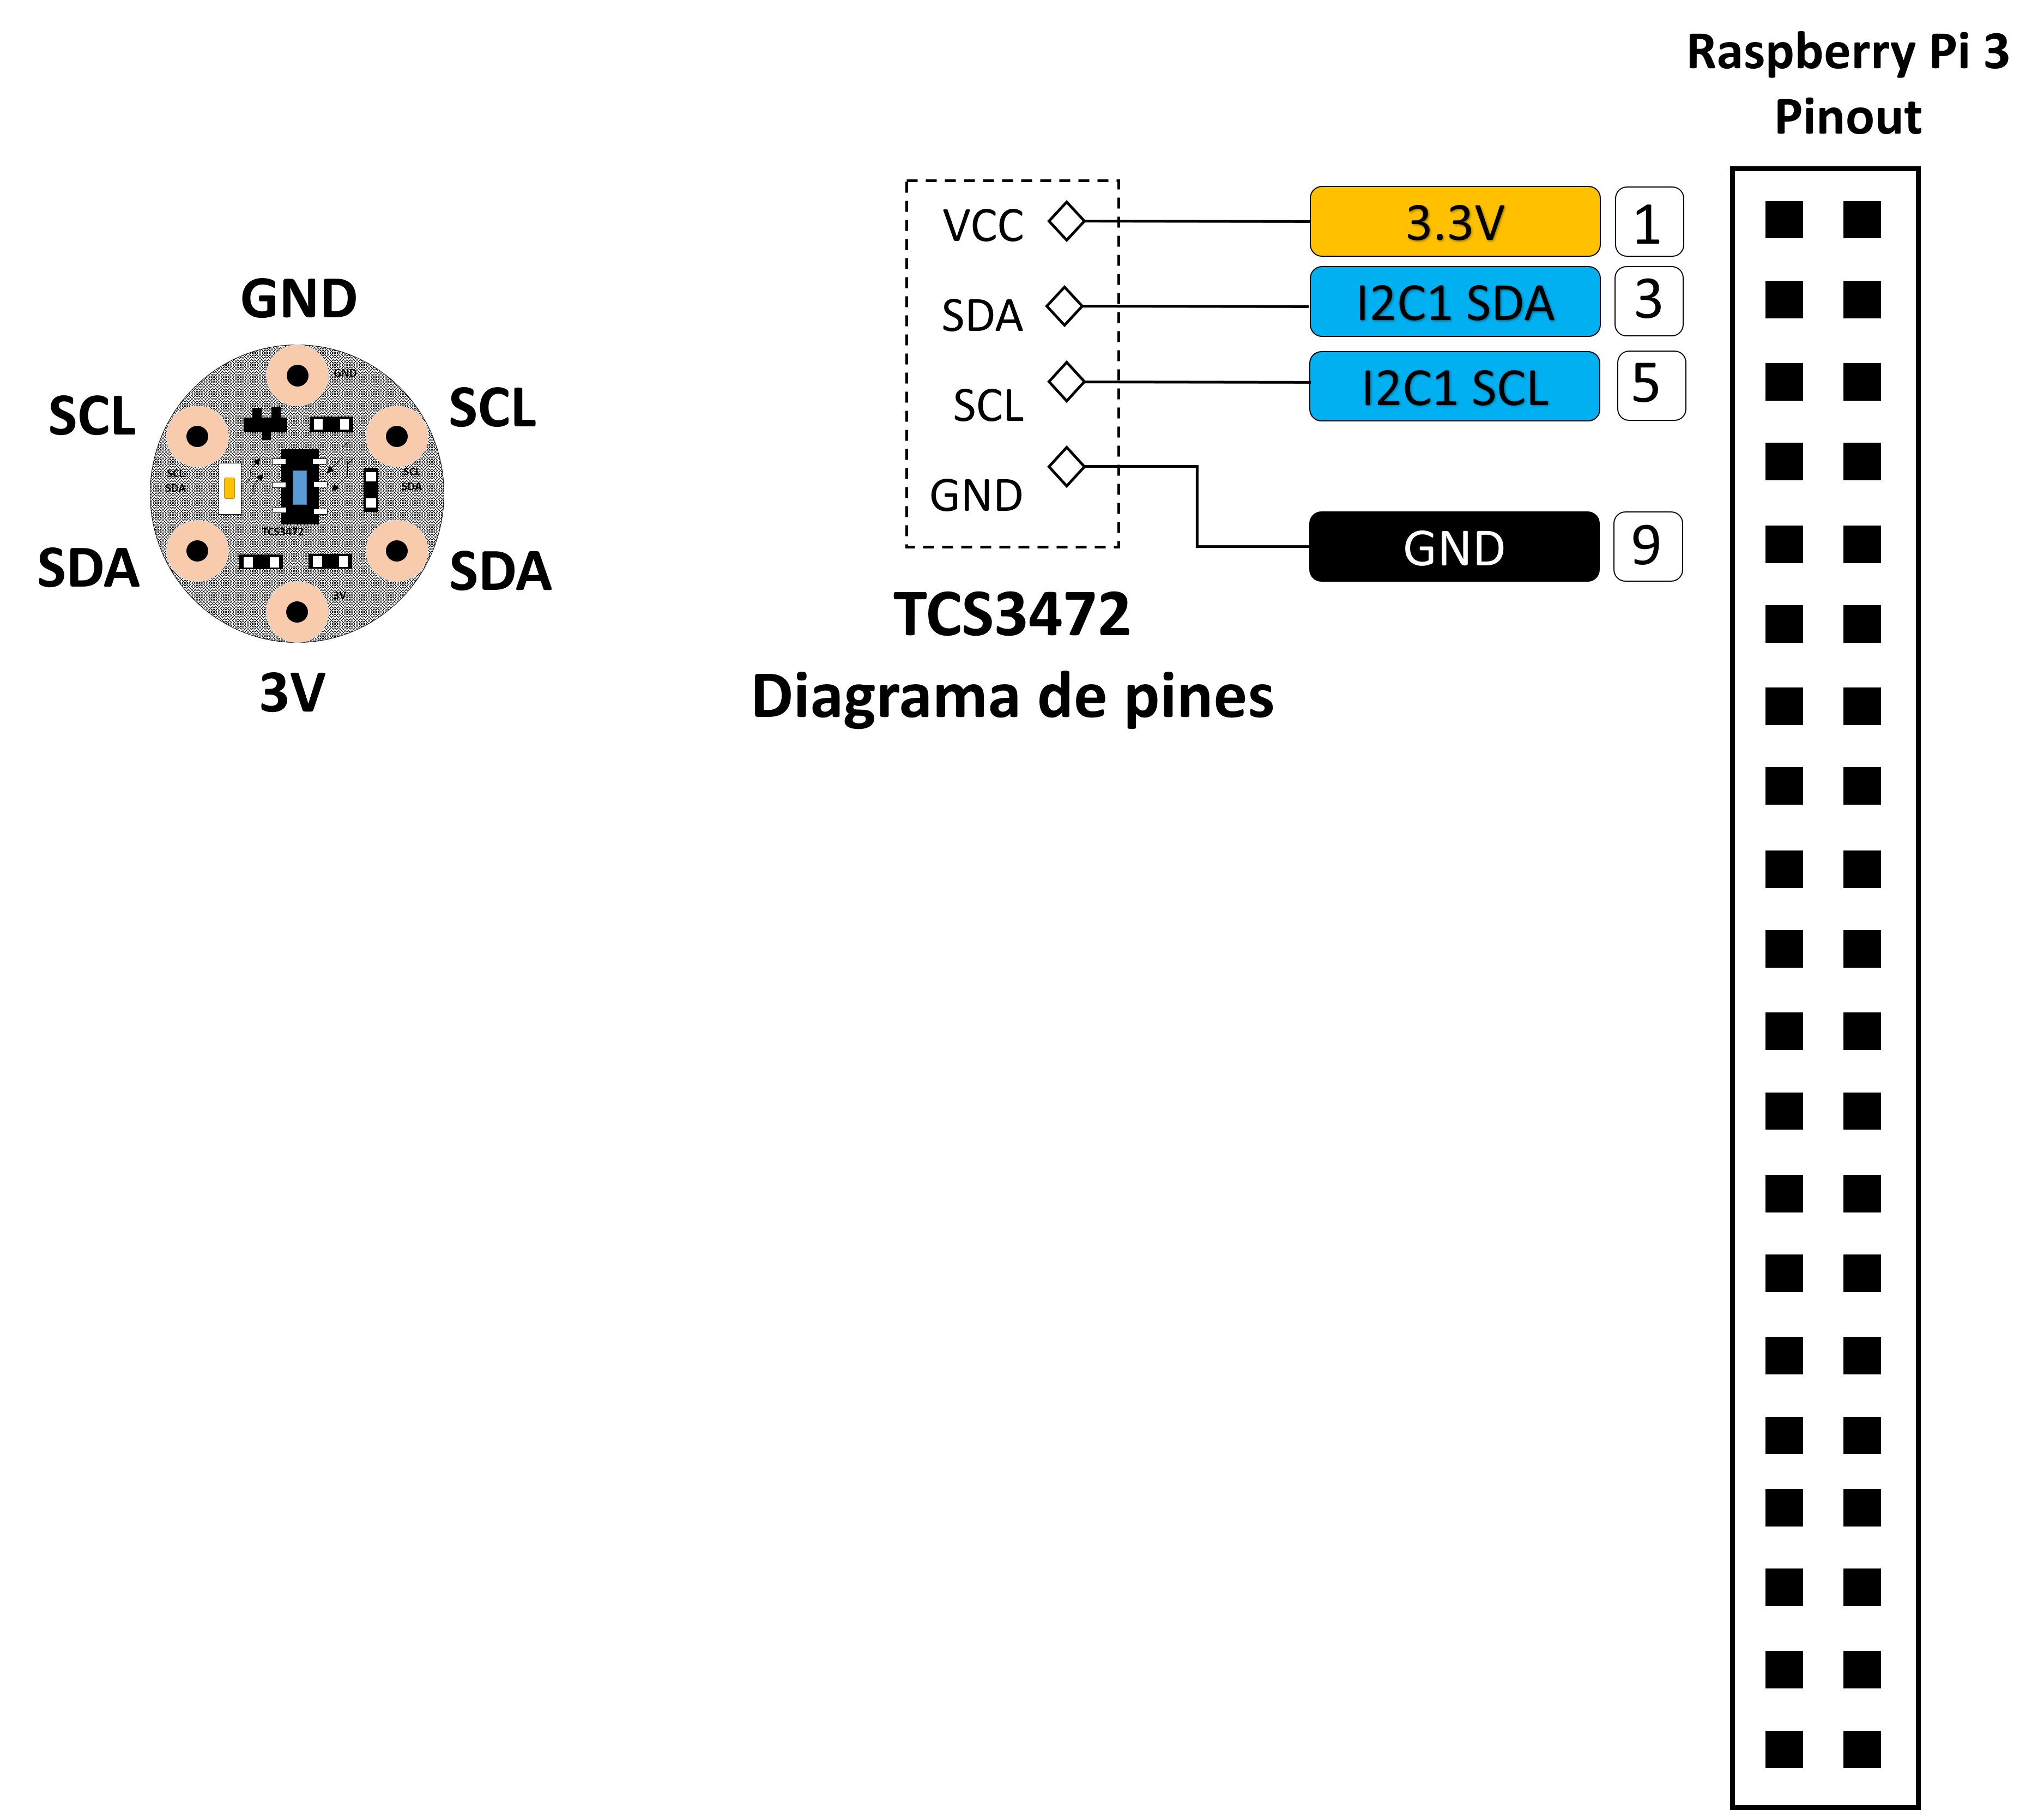
\includegraphics[width=1\textwidth]{color_pinout.png}
\caption{Conexionado TCS34725 Bus I2C con Raspberry Pi.}
\label{fig:conexioncolor}
\end{center}
\end{figure}



\subsubsection{Configuración y lectura, de las posiciones de memoria TCS3472.}

Para establecer comunicaciones mediante \emph{Bus I2C}, entre \emph{Raspberry Pi} y el \emph{sensor TCS3472}, es necesario importar la librería: \texttt{smbus}

Las comunicaciones con el \emph{Bus I2C}, son ejecutadas instanciando el objeto de de clase: \texttt{bus2 = smbus.SMBus(1)}

Para leer datos de los registros de memoria, se utiliza el método: \texttt{bus2.read\_byte\_data()}. Los argumentos de entrada del método son la dirección de memoria del dispositivo, y la dirección del registro que se desea leer.

Para la escritura de datos, se emplea el método: \texttt{bus2.write\_byte\_data()}, que toma como argumentos de entrada la dirección del dispositivo, la dirección a la que se desea acceder, y el valor a escribir en la dirección de memoria.

La dirección por defecto del sensor \emph{TCS3472} es: \texttt{0x29}













\section{Diseño de las aplicaciones.}

\subsection{Aplicación sensor resistivo.}
\subsubsection{Máquinas de estados finitos sensor resistivo.}


\subsection{Aplicación sensor capacitivo.}
\subsubsection{Máquinas de estados finitos sensor capacitivo.}


\subsection{Aplicación sistema tangible orientada a la programación.}
\subsubsection{Máquinas de estados finitos sistema tangible.}






\section{Pruebas y validaciones de librerías y módulos.}




